\documentclass[UTF8,a4paper,11pt,fontset=none]{ctexart}

% ---------- 页面与字体 ----------
\usepackage{geometry}
\geometry{left=2.15cm,right=2.15cm,top=2.35cm,bottom=2.15cm,headsep=0.45cm,footskip=0.95cm}
\usepackage{fontspec}
\setmainfont{texgyretermes}[Extension=.otf,UprightFont=*-regular,BoldFont=*-bold,ItalicFont=*-italic,BoldItalicFont=*-bolditalic]
\setsansfont{texgyreheros}[Extension=.otf,UprightFont=*-regular,BoldFont=*-bold,ItalicFont=*-italic,BoldItalicFont=*-bolditalic]
\setmonofont{Menlo}[Scale=0.84]
\setCJKmainfont{Songti SC}[BoldFont=Songti SC Bold]
\setCJKsansfont{Heiti SC}
\setCJKmonofont{Heiti SC}
\setCJKfamilyfont{zhhei}{Heiti SC}
\setCJKfamilyfont{zhsong}{Songti SC}[BoldFont=Songti SC Bold]
\newcommand{\heiti}{\CJKfamily{zhhei}}
\newcommand{\songti}{\CJKfamily{zhsong}}

% ---------- 通用宏包 ----------
\usepackage{amsmath,amssymb}
\usepackage[table]{xcolor}
\usepackage{graphicx}
\usepackage{booktabs}
\usepackage{tabularx}
\usepackage{array}
\usepackage{multirow}
\usepackage{enumitem}
\usepackage{caption}
\usepackage{subcaption}
\usepackage{fancyhdr}
\usepackage{titlesec}
\usepackage[most]{tcolorbox}
\usepackage{listings}
\usepackage{fontawesome5}
\usepackage{needspace}
\usepackage{float}
\usepackage{hyperref}
\usepackage{tikz}
\usetikzlibrary{arrows.meta,positioning,shapes.geometric,fit,backgrounds,calc}

% ---------- 颜色 ----------
\definecolor{ink}{HTML}{111827}
\definecolor{ink2}{HTML}{1F2937}
\definecolor{muted}{HTML}{6B7280}
\definecolor{accent}{HTML}{2563EB}
\definecolor{accent2}{HTML}{0E7490}
\definecolor{gold}{HTML}{B58B2A}
\definecolor{rule}{HTML}{D9DEE8}
\definecolor{codebg}{HTML}{F7F8FA}
\definecolor{navy}{HTML}{0A1020}
\definecolor{soft}{HTML}{F5F7FB}
\definecolor{warm}{HTML}{B45309}

% ---------- 标题样式 ----------
\titleformat{\section}[block]
  {\centering\heiti\Large\color{ink}}
  {\thesection}{0.7em}{}
\titleformat{\subsection}
  {\heiti\Large\color{ink2}}
  {\thesubsection}{0.6em}{}
\titleformat{\subsubsection}
  {\heiti\normalsize\color{ink2}}
  {\thesubsubsection}{0.5em}{}
\titlespacing*{\section}{0pt}{13pt plus 2pt minus 2pt}{8pt}
\titlespacing*{\subsection}{0pt}{10pt plus 1pt minus 1pt}{5pt}
\titlespacing*{\subsubsection}{0pt}{6pt plus 1pt minus 1pt}{3pt}

% ---------- 页眉页脚 ----------
\setlength{\headheight}{22pt}
\pagestyle{fancy}
\fancyhf{}
\fancyhead[L]{\small\color{muted}StellarLit · 论文星图}
\fancyhead[R]{\small\color{muted}技术文档}
\fancyfoot[C]{\small\color{muted}\thepage}
\renewcommand{\headrulewidth}{0pt}

% ---------- 段落与浮动 ----------
\linespread{1.15}
\setlength{\parindent}{2em}
\setlength{\parskip}{0.18em plus 0.06em}
\setlength{\emergencystretch}{2em}
\tolerance=3000
\setcounter{tocdepth}{1}
\setcounter{secnumdepth}{3}
\renewcommand{\arraystretch}{1.28}
\setlength{\heavyrulewidth}{0.9pt}
\setlength{\lightrulewidth}{0.45pt}
\arrayrulecolor{ink}
\setlength{\tabcolsep}{6pt}
\captionsetup{font=small,labelfont={bf,color=accent},labelsep=quad,skip=4pt}
\setlist[itemize]{leftmargin=2em,itemsep=2pt,topsep=3pt,parsep=0pt}
\setlist[enumerate]{leftmargin=2.2em,itemsep=2pt,topsep=3pt,parsep=0pt}
\renewcommand{\figurename}{图}
\renewcommand{\tablename}{表}
\renewcommand{\contentsname}{目\quad 录}
\renewcommand{\refname}{参考文献}

% ---------- 表格列型 ----------
\newcolumntype{L}[1]{>{\raggedright\arraybackslash}p{#1}}
\newcolumntype{C}[1]{>{\centering\arraybackslash}p{#1}}
\newcolumntype{Y}{>{\raggedright\arraybackslash}X}

% ---------- 代码 ----------
\lstdefinestyle{code}{
  backgroundcolor=\color{codebg},
  basicstyle=\ttfamily\footnotesize,
  keywordstyle=\color{accent}\bfseries,
  commentstyle=\color{muted},
  stringstyle=\color{accent2},
  frame=single,
  rulecolor=\color{rule},
  framerule=0.4pt,
  breaklines=true,
  columns=fullflexible,
  keepspaces=true,
  showstringspaces=false,
  numbers=left,
  numberstyle=\tiny\color{muted},
  numbersep=7pt,
  xleftmargin=1.4em,
  framexleftmargin=0.9em,
  aboveskip=5pt,
  belowskip=5pt
}
\lstset{style=code}

% ---------- 提示框 ----------
\newtcolorbox{keybox}[1]{
  enhanced,breakable=false,
  colback=accent!4,colframe=accent!55,
  boxrule=0.5pt,arc=1.6mm,
  left=3.5mm,right=3.5mm,top=2.2mm,bottom=2.2mm,
  fontupper=\small,
  title={\heiti\small #1},fonttitle=\bfseries,coltitle=ink2,
  attach boxed title to top left={xshift=2mm,yshift=-2mm},
  boxed title style={colback=accent!10,colframe=accent!55,arc=1mm,boxrule=0.4pt}
}
\newtcolorbox{designbox}[1]{
  enhanced,breakable,
  colback=soft,colframe=rule,
  boxrule=0.4pt,arc=1.4mm,
  left=3.5mm,right=3.5mm,top=2mm,bottom=2mm,
  title={\heiti\small #1},fonttitle=\bfseries,
  coltitle=ink2,
  attach boxed title to top left={xshift=2mm,yshift=-2mm},
  boxed title style={colback=white,colframe=rule,arc=1mm,boxrule=0.4pt}
}
\newtcolorbox{warnbox}[1]{
  enhanced,breakable,
  colback=warm!4,colframe=warm!45,
  boxrule=0.4pt,arc=1.2mm,
  left=3.5mm,right=3.5mm,top=2mm,bottom=2mm,
  title={\heiti\small #1},fonttitle=\bfseries,
  coltitle=warm
}

% ---------- 行内代码 ----------
\newcommand{\code}[1]{\texttt{\detokenize{#1}}\allowbreak}
\newcommand{\en}[1]{{\rmfamily #1}}

% ---------- 超链接 ----------
\hypersetup{
  colorlinks=true,
  linkcolor=accent,
  urlcolor=accent,
  citecolor=accent,
  pdftitle={StellarLit 论文星图技术文档},
  pdfauthor={西安交通大学 白白BAB},
  pdfsubject={2026 第九届传智杯 AI WEB 网页开发挑战赛 赛道 10037}
}

\graphicspath{{../screenshots/}}

\begin{document}

\begin{titlepage}
\thispagestyle{empty}
\begin{tikzpicture}[remember picture,overlay]
  % 整页星图背景（左侧已烘焙深色渐隐，保证文字对比度）
  \node[inner sep=0pt] at (current page.center)
    {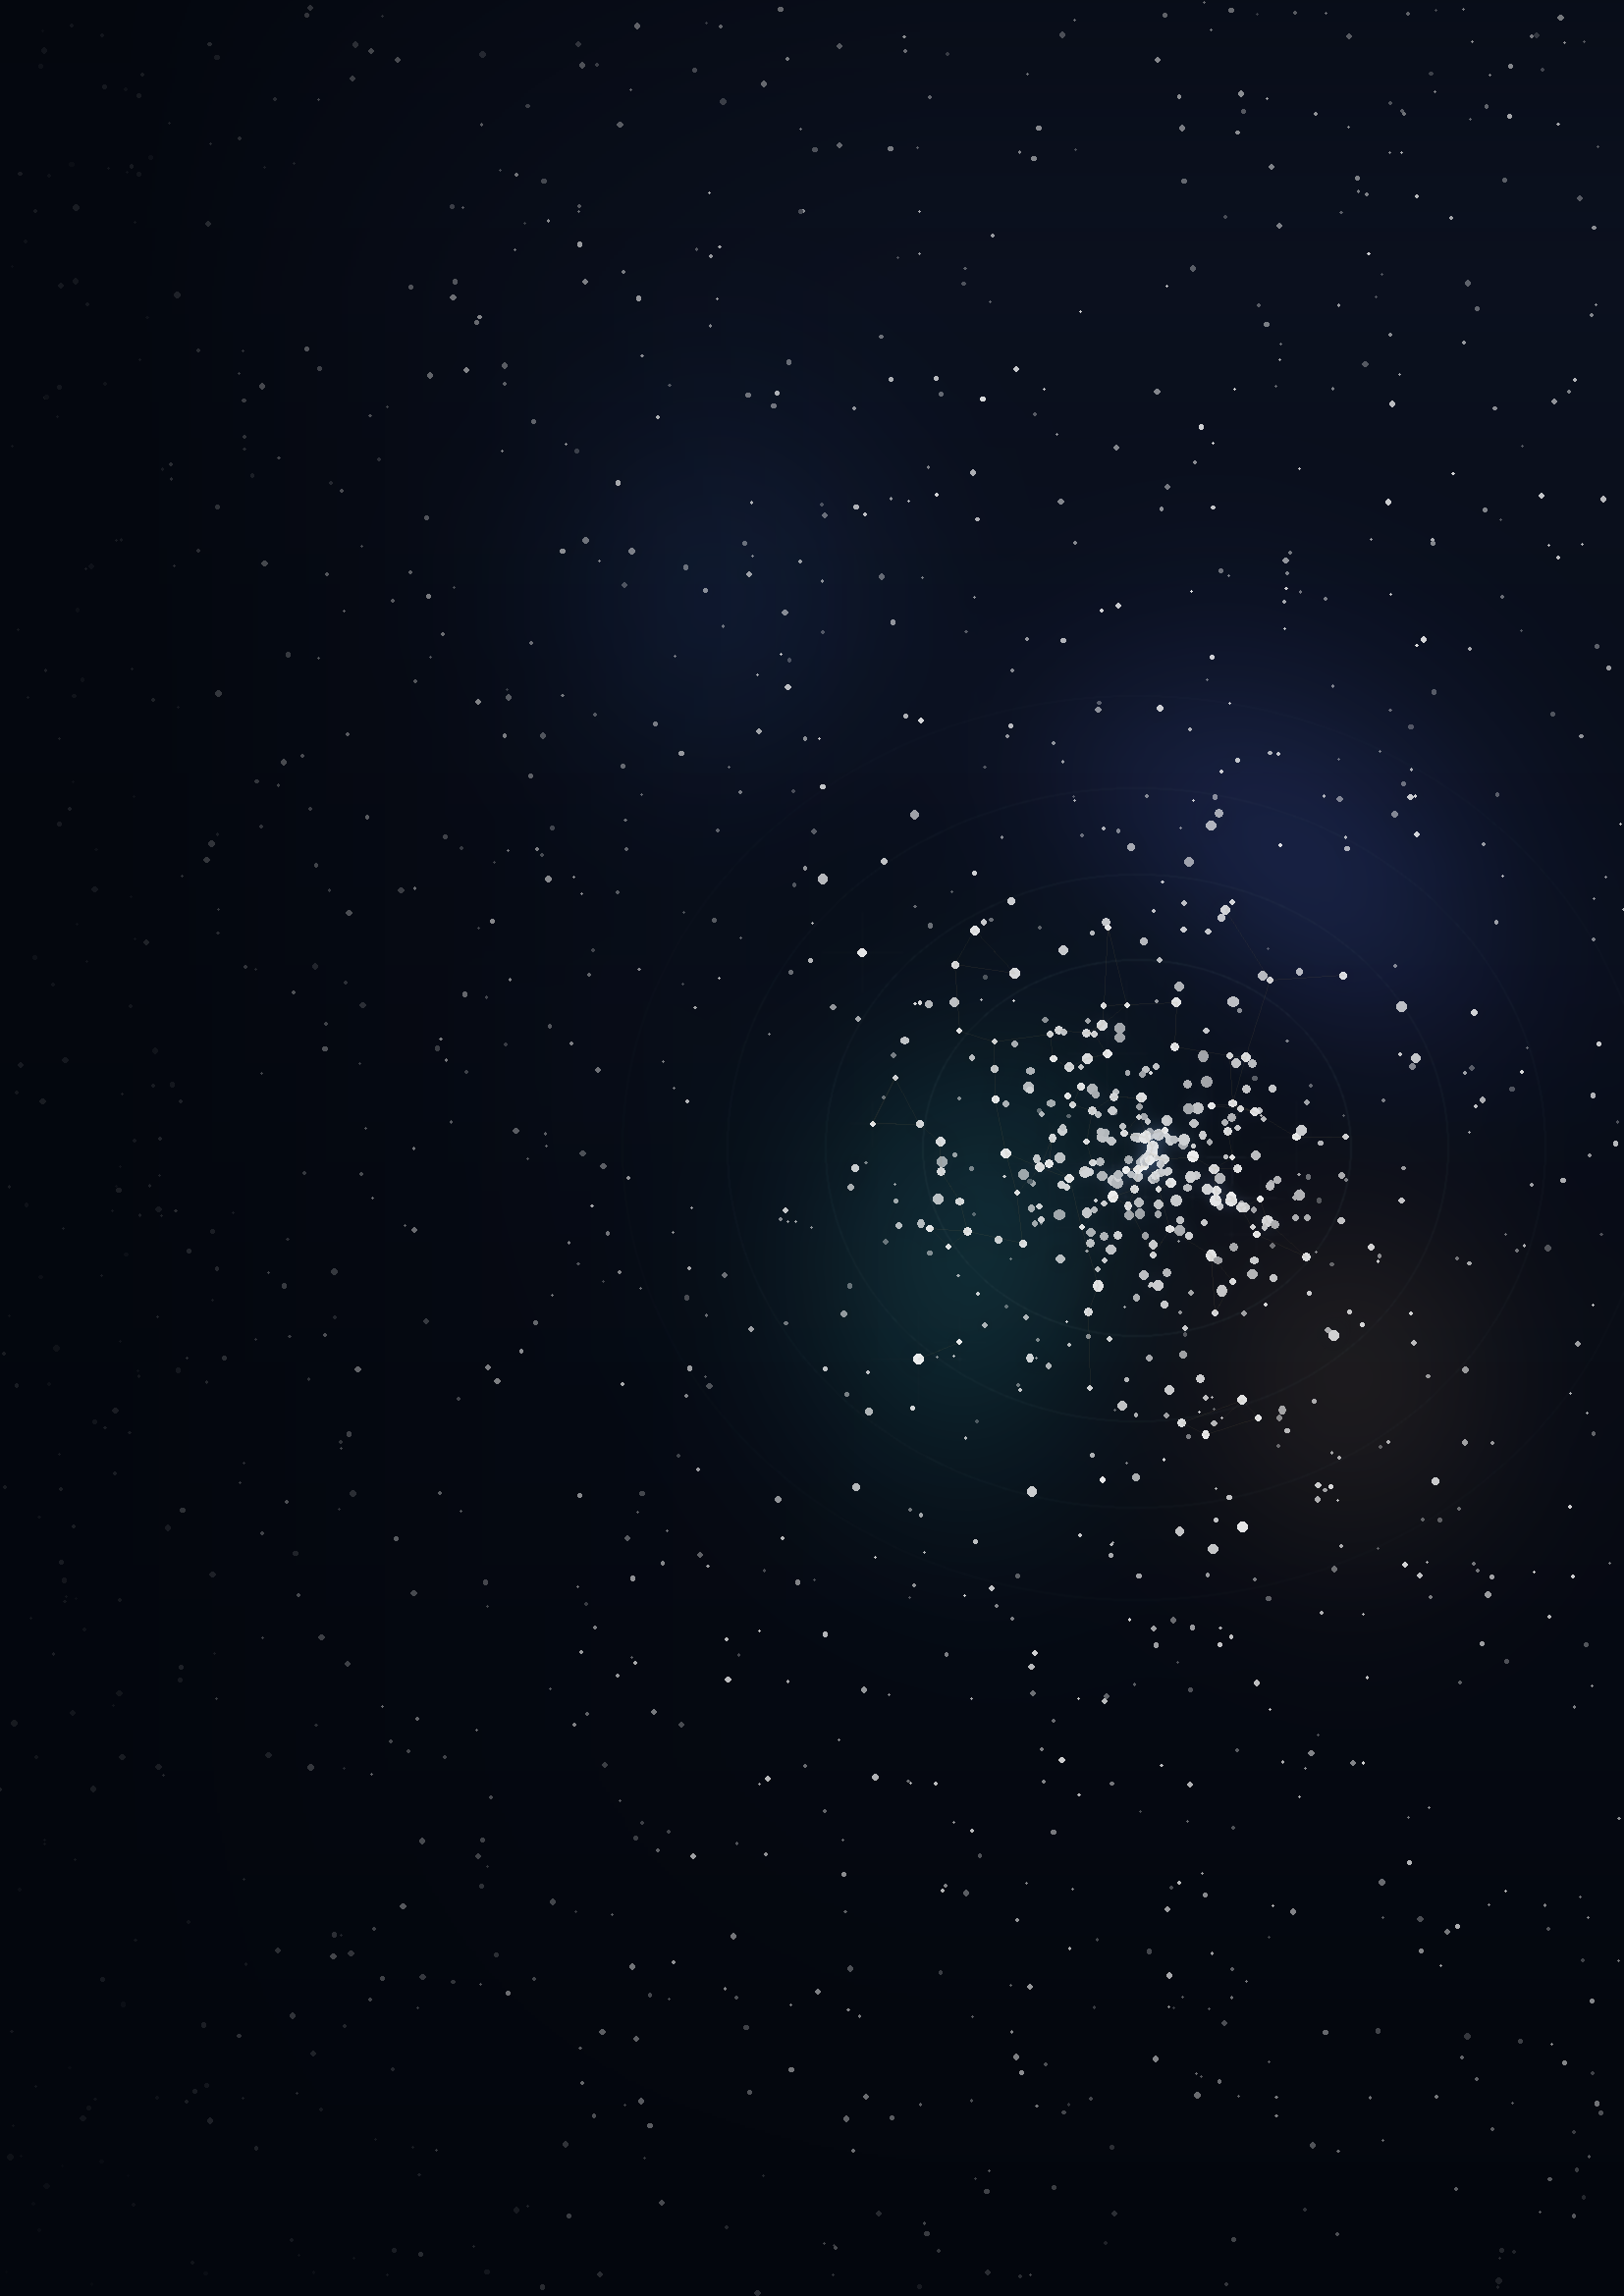
\includegraphics[width=\paperwidth,height=\paperheight]{figures/cover-bg.png}};

  % 顶部赛事标识
  \node[anchor=north west,text width=15.5cm,align=left]
    at ([xshift=2.15cm,yshift=-1.85cm]current page.north west)
    {\color{white!90}\heiti\small 2026 第九届“传智杯”全国大学生数智创新与 AI 应用大赛\\
     \color{white!62}\footnotesize AI WEB 网页开发挑战赛 · 赛道 10037 · RAG 知识问答系统};

  % 主标题
  \node[anchor=west,text width=14cm,align=left]
    at ([xshift=2.15cm,yshift=1.72cm]current page.west)
    {\color{white}\heiti\fontsize{47}{55}\selectfont StellarLit};
  \node[anchor=west,text width=14cm,align=left]
    at ([xshift=2.15cm,yshift=0.55cm]current page.west)
    {\color{white!95}\heiti\fontsize{25}{32}\selectfont 论文星图};
  \node[anchor=west,text width=14cm,align=left]
    at ([xshift=2.15cm,yshift=-0.55cm]current page.west)
    {\color{gold}\heiti\fontsize{16}{22}\selectfont 技术文档};

  \draw[gold,line width=0.8pt] ([xshift=2.15cm,yshift=-1.35cm]current page.west) -- ++(4.2cm,0);

  \node[anchor=west,text width=11.6cm,align=left]
    at ([xshift=2.15cm,yshift=-2.35cm]current page.west)
    {\color{white!92}\large 把一篇论文，长成一片星空。\\[4pt]
     \color{white!74}\normalsize 可核验的关系图谱 · 可追问的文献工作台};

  % 底部信息
  \node[anchor=south west,text width=15.6cm,align=left]
    at ([xshift=2.15cm,yshift=1.45cm]current page.south west)
    {\color{white!94}\heiti\normalsize 西安交通大学 · 白白 BAB · 研究生组\\[3pt]
     \color{white!72}\small 指导教师：白秀秀\quad|\quad 队员：薛志恒（队长）、张子桦、陈林涛};
  \node[anchor=south east]
    at ([xshift=-2.15cm,yshift=1.45cm]current page.south east)
    {\color{white!68}\small v1.0 · 2026 年 11 月};
\end{tikzpicture}
\end{titlepage}

\thispagestyle{plain}
\begin{center}
  {\heiti\LARGE 摘\quad 要}\\[2pt]
  {\color{rule}\rule{3.2cm}{0.7pt}}
\end{center}
\vspace{0.5em}

\addcontentsline{toc}{section}{摘要}

科研文献调研的核心困难，不是“找不到论文”，而是“看得见引用，却看不见为什么相关”。传统检索把论文排成列表，引用网络只回答“谁引用了谁”，通用问答模型又很难为每一句结论给出可核验的出处。StellarLit（论文星图）试图把这三件事接起来：输入标题、DOI 或 arXiv ID，系统从 OpenAlex、arXiv 与 Semantic Scholar 展开引文邻域，用大模型判定论文之间的六类语义关系，并把结果组织成一张可缩放、可点选、可追问的星图。

系统以三层知识图谱为数据契约：L1 结构层保存可公开核验的引用与发表事实，L2 语义层由大模型生产且每条边必须携带原文证据，L3 派生层由社区检测、模块度择优与布局算法生成。AI 方案围绕“可信”与“可控成本”展开：关系判定采用“确定性硬约束过滤 + 多标签 rubric 判定 + 引用片段核验”的两段式管道；问答采用 BM25 与向量双路召回、RRF 融合、图结构扩展与意图重排；Agent 只负责规划“下一步查什么”，停止条件由可复现的覆盖率规则判定；多模态模型把图表转成带归一化坐标的证据块；MCP 则把星空开放为 9 个只读工具，供外部 Agent 复用。

工程上，项目采用 Next.js 15、React 19、TypeScript strict、PostgreSQL 16、Redis 7 与 Docker Compose，前端负责渲染与交互，Route Handlers 只承担 AI 接入与轻量持久化。仓库内置 15 项可重复自检，覆盖类型、规范、RAG、Agent、安全、加密、缓存、数据库与账号隔离。本文档按项目概述、需求分析、系统架构设计、AI 技术方案、核心功能实现、测试与部署、创新点与总结展望展开，并给出关键参数、失败降级路径与已知边界。

\vspace{0.6em}
\begin{keybox}{一句话概括}
StellarLit 不是“另一个论文搜索框”，而是一张\textbf{可核验、会长大、能对话}的研究星图：关系有证据，调研能累积，结论可回溯。
\end{keybox}

\vspace{0.2em}
\noindent\textbf{关键词：} 文献图谱；检索增强生成；多标签关系判定；Agent 工作流；多模态；MCP；可解释 AI

\vfill
\begingroup
\parindent=0pt
\noindent\begin{minipage}{\textwidth}
{\heiti\small 文档信息}\par
\vspace{2pt}
{\color{rule}\rule{\textwidth}{0.4pt}}\par
\vspace{2pt}
\renewcommand{\arraystretch}{1.35}
\begin{tabular}{@{}>{\raggedright\arraybackslash}p{2.8cm}>{\raggedright\arraybackslash}p{\dimexpr\textwidth-2.8cm-14pt\relax}@{}}
项目名称 & StellarLit · 论文星图 \\
参赛赛事 & 2026 第九届“传智杯”全国大学生数智创新与 AI 应用大赛 \\
赛道方向 & AI WEB 网页开发挑战赛 · 赛道 10037 · RAG 知识问答系统（学术文献助手） \\
团队信息 & 西安交通大学 · 白白BAB · 研究生组 \\
指导教师 & 白秀秀 \\
文档版本 & v1.0，2026 年 11 月 16 日 \\
代码仓库 & \href{https://github.com/Xuezhihengg/stellarlit}{GitHub · Xuezhihengg/stellarlit} \\
\end{tabular}
\end{minipage}
\endgroup

\newpage

\thispagestyle{plain}
\tableofcontents

\vfill
\begin{designbox}{阅读导引}
\begin{tabularx}{\textwidth}{L{4.2cm}Y}
第 1--2 章 & 项目要解决什么问题、为谁解决、需求如何被验收。\\
第 3 章 & 分层架构、技术选型、图谱数据契约与 Canvas 渲染管线。\\
第 4 章 & AI 选型理由、集成方式与优化策略，是本文档的技术重点。\\
第 5 章 & 种子解析、星空生长、关系证据、RAG 问答、多模态与 MCP 的实现。\\
第 6--7 章 & 15 项自检、Docker 部署、安全边界，以及创新点与后续路线。\\
\end{tabularx}
\end{designbox}

\newpage


\section{项目概述}

\subsection{背景：文献调研中的三重断裂}

过去十年，学术文献的检索入口越来越顺滑，但“检索”与“理解”之间的缝隙并没有缩小。一个刚进入新方向的研究生，通常会在一天之内经历三次断裂。

\begin{enumerate}
  \item \textbf{列表与结构之间的断裂。} 搜索引擎给出的是按相关度排序的标题列表；引用数据库给出的是有向的引用边。前者丢失了论文之间的关系，后者只说明“谁引用过谁”，却说不清“为什么这两篇值得放在一起读”。
  \item \textbf{关系与证据之间的断裂。} 通用问答模型可以流畅地总结一篇论文，但它的结论往往没有落点：用户看到“A 是 B 的基线”，却无法点回原文，确认这句话究竟来自摘要、引言，还是模型根据常识补出来的。
  \item \textbf{一次检索与长期调研之间的断裂。} 大多数工具把一次查询当成一次会话的终点。用户今天查一个方向，明天补两篇新论文，之前的图、笔记与问题很难继续生长；每次重新搜索，都像重新开始。
\end{enumerate}

我们认为，文献调研真正缺的不是“更多结果”，而是一张\textbf{能被质疑、能被累积、能被追问}的关系地图。StellarLit 因此把“论文”当作星体，把“关系”当作引力线：输入一篇种子论文，沿着引用与语义关系长出一片星空；每条边都带原文证据，每次回答都能点回出处。

\subsection{项目定位：从检索列表到研究星图}

StellarLit 的定位可以拆成三个转变。

\begin{itemize}
  \item \textbf{从“列表”到“星图”。} 论文不是一个孤立的条目，而是某个社区、某个领域中的节点。系统用三层图谱把结构事实、语义推断与算法派生分开表达，让用户既能看见局部论文，也能拉远看见领域星云。
  \item \textbf{从“引用”到“关系 + 证据”。} 除引用外，系统判定基线、同期、思路类似、同任务异方法、扩展、结论矛盾六类语义关系；每一类都有判定标准、反例与硬约束，每条语义边必须携带至少一条能指回原文的证据。
  \item \textbf{从“一次性问答”到“可生长的研究台”。} 同一片星空可以反复并入新种子，老节点坐标保持稳定；问答历史、决策轨迹与图像证据都被保留，用户可以回到上次的研究现场继续追问。
\end{itemize}



\subsection{设计目标}

\begin{table}[H]
  \centering
  \footnotesize
  \caption{StellarLit 的四项设计目标与可观察行为}
  \label{tab:goals}
  \begin{tabularx}{\textwidth}{L{2.6cm}L{5.6cm}Y}
    \toprule
\textbf{目标} & \textbf{含义} & \textbf{用户能观察到的行为} \\
    \midrule
    可信 & 结论有出处，推断可复核 & 点开任意语义边，看到关系类型、置信度与原文片段；回答中的角标可定位到论文与文本块 \\
    可长大 & 调研过程可累积，而非一次一图 & 同一片星空可多次并入种子；老星体不漂移，历史星空可一键回到上次视角 \\
    可对话 & 不只展示图，还能围绕图提问 & 流式回答、比较类问题拆解、证据不足时自动补查，并展示“为什么停” \\
    可扩展 & 能力不只服务站内页面 & 9 个只读 MCP 工具，外部 Agent 可读取星空、检索原文、查证关系 \\
    \bottomrule
  \end{tabularx}
\end{table}

\subsection{功能概览}

\begin{table}[H]
  \centering
  \caption{核心能力与实现要点}
  \label{tab:features}
  \begin{tabularx}{\textwidth}{L{3.1cm}L{4.6cm}Y}
    \toprule
\textbf{能力} & \textbf{用户入口} & \textbf{实现要点} \\
    \midrule
    种子解析 & 标题 / DOI / arXiv ID & 永远返回候选列表，由用户确认；候选带置信度与推荐理由，不替用户做决定 \\
    星空生长 & 选择候选后自动构建 & 展开引文邻域，去重、建图、社区检测、服务端布局；老节点作为锚点参与增量松弛 \\
    关系判定 & 构建时自动执行，可在设置页调整 & 硬约束预过滤 + 多标签 rubric 判定 + 引用片段核验；每条语义边带证据 \\
    证据查看 & 点击星体或关系边 & 展示摘要、关系类型、置信度、原文片段；边有固定的视觉编码 \\
    文献问答 & 底部观星台输入问题，可附 4 张图 & 混合检索 + Agent 补查 + SSE 流式回答；角标回原文，图像证据可定位 \\
    历史与账号 & 左侧历史、账号菜单 & 星空、问答历史、模型配置、用量与 MCP 令牌按账号隔离 \\
    模型服务 & 设置页按账号绑定 & 多厂商 OpenAI 兼容接口；判定 / 问答 / 翻译 / 向量模型分别选择 \\
    MCP & 设置页生成个人令牌 & 9 个只读工具，stdio 与 HTTP 双入口，外部 Agent 即插即用 \\
    \bottomrule
  \end{tabularx}
\end{table}

\subsection{与赛题要求的对应}

赛题强调“前端 Web 应用为主要呈现形态，后端服务仅作为 AI 能力的接入层”，并要求覆盖大模型集成、Agent 工作流、RAG、多模态、AI 安全与 MCP 等能力。本项目没有另起一套独立后端，而是把 AI 接入、轻量持久化与协议入口收敛在 Next.js 的 Route Handlers 中；图谱渲染、交互与 AI 决策轨迹仍在 Web 应用一侧完成。

\begin{table}[H]
  \centering
  \scriptsize
  \caption{赛题能力项与本项目实现的对应关系}
  \label{tab:contest}
  \begin{tabularx}{\textwidth}{L{3.4cm}L{7.2cm}L{2.4cm}}
    \toprule
\textbf{赛题能力} & \textbf{本项目实现} & \textbf{详见} \\
    \midrule
    大模型集成 & 多厂商 OpenAI 兼容接口 + Anthropic 适配；结构化 JSON 判定、SSE 流式回答、超时 / 限流 / 余额不足的可读降级 & 第 4.2--4.3 节 \\
    Agent 工作流 & 规划 → 工具调用 → 证据覆盖判定 → 补查或停止；最多 2 轮 / 5 步，界面留下完整决策轨迹 & 第 4.6 节 \\
    RAG & 摘要与关系原文切块；BM25 + 向量双路召回；RRF 融合、图结构扩展、意图重排与证据阈值 & 第 4.5 节 \\
    多模态 & 最多 4 张图；视觉模型抽取 OCR、表格、图表序列、关键数值与归一化区域坐标 & 第 4.7 节 \\
    AI 安全 & 输入净化、资料与指令隔离、IP 限流与并发上限、每日 token 预算、输出兜底 & 第 4.8 节 \\
    MCP & 9 个只读工具，个人访问令牌，stdio 与 HTTP 双入口 & 第 5.6 节 \\
    前端工程 & Next.js 15 + React 19 + TypeScript strict；Canvas 2D 自写渲染管线；ESLint 强制依赖单向 & 第 3 章 \\
    \bottomrule
  \end{tabularx}
\end{table}

\needspace{4\baselineskip}
\section{需求分析}

\subsection{用户画像与典型场景}

StellarLit 面向的不是“随便搜一篇论文”的泛用户，而是需要在一个方向上建立结构认知、并且愿意核对出处的科研读者。下表列出三类典型用户与他们的关键诉求。

\begin{table}[htbp]
  \centering
  \caption{用户画像与关键诉求}
  \label{tab:persona}
  \begin{tabularx}{\textwidth}{L{3.0cm}L{5.5cm}Y}
    \toprule
\textbf{用户} & \textbf{典型任务} & \textbf{最在意什么} \\
    \midrule
    低年级研究生 & 进入新方向，读第一篇综述后想快速搭骨架 & 哪些是基线、哪些是同期工作、哪些结论互相矛盾；每条判断能否核对原文 \\
    交叉方向研究者 & 把本领域方法迁移到另一个任务 & 同一思路在不同任务上的对应工作；“同任务异方法”与“思路类似”能否区分 \\
    教师 / 评审 & 快速理解一个项目或方向的谱系 & 图谱是否稳定、能否复现；结论是否有证据，而不是模型自由发挥 \\
    \bottomrule
  \end{tabularx}
\end{table}

一个完整场景如下：用户输入 \emph{Attention Is All You Need}，系统返回若干候选并说明推荐理由；用户确认后，星空以该论文为锚点展开向前与向后的引文邻域，判定出“基线 / 扩展 / 同任务异方法 / 结论矛盾”等关系。用户点开一条边，看到“B 明确把 A 作为对比对象”的原文片段；随后提问“Transformer 与状态空间模型是什么关系”，系统发现默认检索缺少两篇论文之间的关系证据，自动补查一次，给出带角标的回答，并展示“证据已足够，停止补查”的决策轨迹。用户再把第二篇种子并入同一片星空，老星体留在原位，只长出新分支。

\needspace{3\baselineskip}
\subsection{功能需求}

\begin{table}[H]
  \centering
  \footnotesize
  \renewcommand{\arraystretch}{1.12}
  \caption{功能需求与验收标准}
  \label{tab:fr}
  \begin{tabularx}{\textwidth}{L{1.4cm}L{3.7cm}Y L{1.15cm}}
    \toprule
\textbf{编号} & \textbf{需求} & \textbf{验收标准} & \textbf{优先级} \\
    \midrule
    FR-01 & 种子解析 & 支持标题、DOI、arXiv ID；返回多个候选，含年份、被引量、置信度与推荐理由 & 高 \\
    FR-02 & 候选确认 & 不自动选择；已在本星空中的论文标记为“并入”，而不是重复新增 & 高 \\
    FR-03 & 引文邻域 & 向后取参考文献、向前取引用者；主源失败时整片邻域切换到备用源，id 空间保持一致 & 高 \\
    FR-04 & 语义关系 & 支持六类内置关系与最多 24 条自定义关系；一条边可同时成立多个标签 & 高 \\
    FR-05 & 关系证据 & 语义边至少一条原文证据；引用片段必须能在对应论文文本中找到 & 高 \\
    FR-06 & 增量生长 & 同一星空可多次并入种子；已有节点坐标不变，新节点在邻居重心附近松弛 & 高 \\
    FR-07 & 混合检索 & BM25 与向量双路召回；向量不可用时自动退回词面检索，并在诊断中标注 & 高 \\
    FR-08 & Agent 补查 & 最多 2 轮 / 5 步；证据不足时补查，足够时停止；每个决策可在界面查看 & 高 \\
    FR-09 & 流式问答 & SSE 逐段输出；资料事实带 \code{[n]} 角标，通用知识不加角标 & 高 \\
    FR-10 & 多模态 & 最多 4 张图；抽取 OCR、表格、图表数值与区域坐标；证据可点击定位 & 中 \\
    FR-11 & 历史与账号 & 星空、问答历史、模型配置、用量与 MCP 令牌按账号隔离 & 高 \\
    FR-12 & 模型服务 & 按账号绑定多厂商；判定、问答、翻译、向量模型可分别选择 & 高 \\
    FR-13 & MCP & 9 个只读工具；个人令牌只在创建时返回一次，数据库只存 SHA-256 & 中 \\
    FR-14 & 安全与配额 & 输入护栏、IP 限流、并发上限、每日 token 预算；失败返回可行动提示 & 高 \\
    \bottomrule
  \end{tabularx}
\end{table}

\subsection{非功能需求}

\begin{table}[H]
  \centering
  \footnotesize
  \renewcommand{\arraystretch}{1.12}
  \caption{非功能需求与设计手段}
  \label{tab:nfr}
  \begin{tabularx}{\textwidth}{L{2.2cm}L{5.6cm}Y}
    \toprule
\textbf{维度} & \textbf{目标} & \textbf{设计手段} \\
    \midrule
    渲染性能 & 数百至上千节点下保持流畅交互 & 布局在服务端完成；Canvas 一次绘制；悬浮/选中读写分离；动画按 \code{dt} 计算并封顶 64ms \\
    检索延迟 & 重复提问不重复付费 & 星空语料与 BM25 索引按版本缓存；向量按“供应商 + 文本”缓存；关系结论按 \code{promptVersion} 缓存 \\
    可靠性 & 外部依赖失败时主流程不中断 & Redis 不可用则直连源站；向量不可用退回 BM25；模型不可用保留检索摘录或明确提示 \\
    安全 & 密钥不进入浏览器包，不被日志回显 & \code{src/server} 禁止被客户端引用；API Key 以 AES-256-GCM 加密落库；错误消息只取供应商正文 \\
    可维护 & 改动可被自动检查拦住 & TypeScript strict；ESLint 强制依赖单向；15 项 \code{pnpm check} 直接调用生产代码路径 \\
    成本 & 单次建图与问答成本可见、可调 & 硬约束预过滤、批量判定、摘要截断、关系缓存、每日 token 预算 \\
    兼容 & 桌面与窄屏均可使用 & 语义缩放 + 自适应侧栏；关键操作保留键盘可达路径 \\
    \bottomrule
  \end{tabularx}
\end{table}

\subsection{约束与边界}

\begin{itemize}
  \item \textbf{赛题约束：} 前端 Web 应用为主要呈现形态，后端只作为 AI 能力接入层。项目因此不部署独立业务后端，持久化通过 Route Handlers 与 PostgreSQL / Redis 提供，图谱渲染与 AI 决策轨迹仍在前端完成。
  \item \textbf{数据约束：} 上游依赖 OpenAlex、arXiv 与 Semantic Scholar 的公开 API；OpenAlex 使用账号注册邮箱进入礼貌池。上游字段缺失时，系统按由细到粗的层级回退主题标签，而不是让候选直接归零。
  \item \textbf{证据边界：} 当前语义证据到“摘要 + 关系原文”级别，尚未按章节对 arXiv 全文切块。接入全文后，引用可以精确到章节与字符偏移；这一限制在 README 与本文第 7 章中如实说明。
  \item \textbf{部署边界：} 面向单机自托管场景，未实现连接级多租户行安全策略（RLS），账号隔离依靠仓储层每条 SQL 都带 \code{owner_id}；IP 限流计数在单进程内存中，进程重启归零。
\end{itemize}

\section{系统架构设计}

\subsection{总体架构}

系统按“表现层—接入层—AI 能力层—数据与外设层”组织。浏览器负责渲染、交互与状态；Next.js Route Handlers 负责鉴权、限流、参数校验、SSE 与 AI 调用；AI 能力层由 Agent、关系判定、混合检索、多模态与 MCP 组成；数据层保存账号、星空快照、问答历史、用量与缓存，并连接外部文献源和模型服务。

\begin{figure}[htbp]
\centering
\begin{tikzpicture}[font=\scriptsize,>=Latex,
  box/.style={draw=rule,fill=white,rounded corners=1.2mm,align=center,inner sep=1.8pt,minimum height=7mm},
  band/.style={draw=accent!18,fill=soft,rounded corners=2mm},
  lab/.style={font=\heiti\scriptsize,color=ink2,align=center}]

  % L1
  \node[lab,text width=0.95cm] (l1) at (0.65,8.4) {表现层};
  \node[box,text width=2.55cm] (b1) at (3.7,8.4) {页面与路由\\App Router};
  \node[box,text width=2.55cm] (b2) at (7.0,8.4) {Canvas 星图\\渲染管线};
  \node[box,text width=2.35cm] (b3) at (10.3,8.4) {Zustand\\跨组件状态};
  \node[box,text width=2.45cm] (b4) at (13.65,8.4) {问答面板\\SSE 消费};

  % L2
  \node[lab,text width=0.95cm] (l2) at (0.65,5.9) {接入层};
  \node[box,text width=2.55cm] (c1) at (3.7,5.9) {Route Handlers\\/api/*};
  \node[box,text width=2.35cm] (c2) at (7.0,5.9) {鉴权 / 限流\\预算控制};
  \node[box,text width=2.35cm] (c3) at (10.3,5.9) {Zod 校验\\安全护栏};
  \node[box,text width=2.45cm] (c4) at (13.65,5.9) {SSE / JSON\\文件流};

  % L3
  \node[lab,text width=0.95cm] (l3) at (0.65,3.45) {AI 能力层};
  \node[box,text width=2.15cm] (d1) at (2.95,3.45) {Agent\\规划 / 执行\\评估};
  \node[box,text width=2.15cm] (d2) at (5.7,3.45) {关系判定\\硬约束\\多标签判定};
  \node[box,text width=2.15cm] (d3) at (8.45,3.45) {混合 RAG\\BM25 + 向量\\RRF 融合};
  \node[box,text width=2.15cm] (d4) at (11.2,3.45) {多模态\\图像证据};
  \node[box,text width=2.15cm] (d5) at (13.95,3.45) {MCP\\9 个只读工具};

  % L4
  \node[lab,text width=0.95cm] (l4) at (0.65,0.65) {数据与外设};
  \node[box,text width=2.15cm] (e1) at (2.95,0.65) {PostgreSQL\\账号 / 星空\\历史};
  \node[box,text width=1.95cm] (e2) at (5.55,0.65) {Redis\\TTL / 节流};
  \node[box,text width=1.95cm] (e3) at (8.05,0.65) {data/\\媒体 / 缓存};
  \node[box,text width=2.05cm] (e4) at (10.55,0.65) {模型服务\\LLM / Embedding};
  \node[box,text width=2.35cm] (e5) at (13.45,0.65) {文献源\\OpenAlex / arXiv / S2};

  \begin{scope}[on background layer]
    \node[band,fit=(l1)(b4)] {};
    \node[band,fit=(l2)(c4)] {};
    \node[band,fit=(l3)(d5)] {};
    \node[band,fit=(l4)(e5)] {};
  \end{scope}

  \draw[->,thick,accent!65] (8.1,7.55) -- (8.1,6.75) node[midway,right,font=\tiny,color=muted] {HTTPS + SSE};
  \draw[->,thick,accent!65] (8.1,5.05) -- (8.1,4.30) node[midway,right,font=\tiny,color=muted] {内部调用};
  \draw[->,thick,accent!65] (8.1,2.50) -- (8.1,1.75) node[midway,right,font=\tiny,color=muted] {读写 / 调用};
\end{tikzpicture}
\caption{StellarLit 总体架构：浏览器、Route Handlers、AI 编排与数据外设四层。}
\label{fig:arch}
\end{figure}

架构有一条贯穿全局的约束：\textbf{依赖单向}。\code{types} 只定义数据契约，\code{lib} 只放纯逻辑，\code{components} 只消费 \code{features} 与 \code{lib}，\code{app} 负责组装；\code{server} 只能被 \code{app/api} 引用，绝不允许进入浏览器包。这条约束写进了 \code{eslint.config.mjs}，违反即构建失败。之所以用工具而不是靠文档，是因为“这次先这样、下次再拆”从来不会真的拆。

\begin{figure}[htbp]
\centering
\begin{tikzpicture}[font=\small,>=Latex,
  box/.style={draw=rule,fill=white,rounded corners=1.2mm,align=center,inner sep=3pt,minimum height=8mm},
  note/.style={draw=warm!45,dashed,fill=warm!4,rounded corners=1.2mm,align=center,inner sep=3pt}]
  \node[box,text width=2.0cm] (types) at (1.0,0) {\code{types}\\数据契约};
  \node[box,text width=2.2cm] (lib) at (4.1,0) {\code{lib}\\纯逻辑};
  \node[box,text width=2.6cm] (comp) at (7.4,0) {\code{components}\\展示与交互};
  \node[box,text width=2.2cm] (app) at (10.7,0) {\code{app}\\路由与组装};
  \node[box,text width=2.4cm] (server) at (4.1,-1.55) {\code{server}\\AI 接入与仓储};
  \node[box,text width=2.6cm] (api) at (10.7,-1.55) {\code{app/api}\\Route Handlers};

  \draw[->,thick,accent!65] (types) -- (lib);
  \draw[->,thick,accent!65] (lib) -- (comp);
  \draw[->,thick,accent!65] (comp) -- (app);
  \draw[->,thick,accent!65] (server) -- (api);
  \draw[->,thick,accent!65] (api) -- (app);
  \node[note,text width=8.6cm] at (7.4,-2.55) {ESLint 禁止反向依赖；密钥只存在于 \code{src/server}，不得进入浏览器包};
\end{tikzpicture}
\caption{分层与依赖方向：左侧永远不知道右侧存在，服务端代码不得进入浏览器包。}
\label{fig:deps}
\end{figure}

\needspace{3\baselineskip}
\subsection{技术选型与理由}

\begin{table}[htbp]
  \centering
  \footnotesize
  \caption{主要技术选型与取舍}
  \label{tab:stack}
  \begin{tabularx}{\textwidth}{L{2.5cm}L{4.2cm}Y}
    \toprule
\textbf{层} & \textbf{选型} & \textbf{为什么选它 / 代价是什么} \\
    \midrule
    框架 & Next.js 15（App Router）+ React 19 & 页面与 Route Handlers 同仓，AI 接入层不必另起服务；RSC 降低首屏数据往返。代价是构建内存较高，2G 机器需加 swap \\
    语言 & TypeScript strict & 图谱节点、边、模型输出都有明确契约；\code{unknown} 必须经过 Zod 才能进入业务 \\
    样式 & Tailwind CSS v4（CSS-first \code{@theme}） & 设计令牌即 CSS 变量，换主题等于换一套变量；避免样式与业务状态耦合 \\
    状态 & Zustand & 只有跨组件共享的状态才进 store；高频悬浮/选中不触发整树重渲染 \\
    渲染 & Canvas 2D 自写管线 & 上千节点/边时比 SVG/DOM 稳；绘制是纯函数，可脱离 React 测试。代价是命中检测要自己实现 \\
    数据库 & PostgreSQL 16（\code{pg} + JSONB） & 多账号并发写、事务与行级隔离；星空快照以 JSONB 保存，结构演进成本低 \\
    缓存 & Redis 7（\code{ioredis}） & TTL、跨实例共享、上游 host 节流；不可用时自动降级为进程内节流 \\
    校验 & Zod & 模型 JSON、API 入参、图像区域坐标共用一套 schema；解析失败可定位到字段 \\
    协议 & MCP TypeScript SDK & 复用官方工具注册与传输；HTTP 与 stdio 共用同一份工具定义 \\
    部署 & Docker Compose & 应用、PostgreSQL、Redis 一起编排；反向代理只负责 TLS 与 SSE 不缓冲 \\
    \bottomrule
  \end{tabularx}
\end{table}

\subsection{两条核心数据流}

系统有两条主链路：建图链路把“一篇种子”变成“一片星空”，问答链路把“一个问题”变成“一段带角标的回答”。两条链路共享同一份图谱数据契约与同一套模型配置，但在失败降级上各自独立：建图可以在没有模型时保留结构关系，问答在未绑定模型时明确提示，而不是静默给出不可信答案。

\begin{figure}[htbp]
\centering
\begin{tikzpicture}[font=\footnotesize,>=Latex,
  flowbox/.style={draw=rule,fill=white,rounded corners=1.2mm,align=center,inner sep=2.5pt,minimum height=8mm,text width=2.15cm},
  tag/.style={font=\heiti\scriptsize,color=accent2,anchor=west}]
  % build row
  \node[tag] at (-0.2,1.55) {建图};
  \node[flowbox] (s1) at (2.0,1.2) {种子输入\\标题/DOI/arXiv};
  \node[flowbox] (s2) at (4.55,1.2) {候选解析\\用户确认};
  \node[flowbox] (s3) at (7.1,1.2) {邻域展开\\向前/向后};
  \node[flowbox] (s4) at (9.65,1.2) {建图·聚类\\服务端布局};
  \node[flowbox] (s5) at (12.2,1.2) {关系判定\\证据核验};
  \node[flowbox] (s6) at (14.75,1.2) {持久化\\星图渲染};
  \foreach \a/\b in {s1/s2,s2/s3,s3/s4,s4/s5,s5/s6}
    \draw[->,thick,accent!60] (\a) -- (\b);

  % ask row
  \node[tag] at (-0.2,-1.35) {问答};
  \node[flowbox] (q1) at (2.0,-1.7) {问题 + 图像\\最多 4 张};
  \node[flowbox] (q2) at (4.55,-1.7) {安全护栏\\限流/预算};
  \node[flowbox] (q3) at (7.1,-1.7) {初始规划\\JSON 选工具};
  \node[flowbox] (q4) at (9.65,-1.7) {工具检索\\补查/扩展};
  \node[flowbox] (q5) at (12.2,-1.7) {覆盖判定\\确定性停止};
  \node[flowbox] (q6) at (14.75,-1.7) {流式回答\\角标/轨迹};
  \foreach \a/\b in {q1/q2,q2/q3,q3/q4,q4/q5,q5/q6}
    \draw[->,thick,accent2!65] (\a) -- (\b);
\end{tikzpicture}
\caption{建图与问答两条主链路：前者重结构与证据，后者重检索、补查与可解释停止。}
\label{fig:flows}
\end{figure}

\subsection{知识图谱数据模型}

图谱不是“节点和边的集合”这么简单。学术文献里存在三种性质完全不同的知识：客观引用事实、语义推断、算法派生。如果把三者塞进一张扁平表，大模型的幻觉和真实引用看起来一样可信，用户想核对时系统也无法回答“你凭什么这么说”。因此本模型按\textbf{可核验程度}分三层，而不是按业务模块分层。

\begin{table}[htbp]
  \centering
  \small
  \caption{三层图谱：生产者、可信度与视觉表达}
  \label{tab:layers}
  \begin{tabularx}{\textwidth}{L{1.5cm}L{4.4cm}L{3.2cm}Y}
    \toprule
\textbf{层} & \textbf{内容} & \textbf{生产者} & \textbf{可信度与视觉} \\
    \midrule
    L1 结构层 & 引用 \code{CITES}、作者 \code{AUTHORED_BY}、发表 \code{PUBLISHED_IN}、提及 \code{MENTIONS} & OpenAlex、arXiv、Semantic Scholar & 权威、可公开核验；极细引力线与星体标签 \\
    L2 语义层 & 基线、同期、思路类似、同任务异方法、扩展、结论矛盾 & 大模型 + 提示词工程 & 不能直接核验，但必须带原文证据；不同关系有固定线型与颜色 \\
    L3 派生层 & 社区、领域、潜在连接 & 标签传播 + 模块度、向量近邻、统计检验 & 全部可复算；缩小时以星团与星云浮现 \\
    \bottomrule
  \end{tabularx}
\end{table}

节点分实体节点与聚合节点。实体节点包括论文、作者、期刊/会议、概念与文本块；聚合节点（社区、领域）没有自己的数据，是算法对实体节点的分组结果，删掉不影响事实层。文本块 \code{chunk} 是 RAG 的检索单元，必须携带 \code{locator}（章节、段落序号或原文偏移），否则模型给出的引用无法回溯——界面上那些角标就会变成不可点击的装饰。

\begin{table}[htbp]
  \centering
  \small
  \caption{六类内置语义关系：硬约束、证据策略与视觉编码}
  \label{tab:relations}
  \begin{tabularx}{\textwidth}{L{2.0cm}L{2.2cm}L{4.3cm}L{2.4cm}Y}
    \toprule
\textbf{关系} & \textbf{关系族} & \textbf{硬约束} & \textbf{证据策略} & \textbf{视觉} \\
    \midrule
    基线 & 谱系 & 必须存在引用；年份差 $\le 8$ & 结构 + 原文 & 带方向实线，粒子表示流向 \\
    扩展 & 谱系 & 必须存在引用；年份差 $\le 10$ & 结构 + 原文 & 带方向实线 \\
    同期 & 对照 & 互不引用；年份差 $\le 2$ & 结构 & 虚线（平行但未交汇） \\
    思路类似 & 对照 & 标题+摘要 TF-IDF 相似度 $\ge 0.15$ & 原文 & 冷色实线 \\
    同任务异方法 & 对照 & 必须共享任务 & 原文 & 双色调对撞线 \\
    结论矛盾 & 冲突 & 必须共享任务 & 原文 & 全图唯一暖红色 \\
    \bottomrule
  \end{tabularx}
\end{table}

写入图之前会校验六条不变式：语义边至少一条证据；结构边必须有上游出处；引用边不得自环且 \code{CITES} 不允许成环；聚合节点不得作为引用端点；同一对节点同一关系只保留置信度最高的一条并合并证据；文本块必须有定位。违反即拒绝入库，而不是静默降级。

\subsection{渲染架构与语义缩放}

系统选择 Canvas 而不是 SVG/DOM，原因不是“Canvas 更酷”，而是节点与边一旦上千，DOM 方案的三类开销会同时出现：内存与样式重算随节点数线性增长；布局一动要做上千次样式计算；悬浮高亮要改上千个类名。Canvas 把这三类开销压成一次绘制调用，代价是要自己实现命中检测——但命中检测本来就带空间语义（命中半径随缩放变化、空白处需要吸附），DOM 的 \code{:hover} 帮不上忙。

三条性能约定贯穿渲染管线：布局在服务端算完，前端只做投影，主线程不跑 $O(n^2)$；悬浮/选中双写，渲染循环读 ref、React 读 state，高频状态不触发重渲染；动画按秒计算而不按帧计数，\code{dt} 上限 64ms，在 120Hz 屏与切标签页回来时都不失真。

\begin{table}[htbp]
  \centering
  \caption{语义缩放：缩放比例对应抽象层级}
  \label{tab:zoom}
  \begin{tabularx}{\textwidth}{L{2.6cm}L{3.2cm}Y}
    \toprule
\textbf{缩放区间} & \textbf{看到什么} & \textbf{读的是哪一层} \\
    \midrule
    \code{scale < 0.34} & 领域星云 + 中文标题 & \code{domain} 聚合节点 \\
    \code{0.34 <= scale < 0.78} & 星团 + 社区标签 & \code{community} 聚合节点 \\
    \code{scale >= 0.78} & 论文星体 + 关系边 & \code{paper} 实体节点与边 \\
    \bottomrule
  \end{tabularx}
\end{table}

增量构建是“星空会长大”的关键。新增种子时，如果整张图重新布局，老星体会整体漂移，用户看到的现象就是“我一搜，原来的星图就没了”。因此世界原点固定在中心，世界只做对称长大；已有节点作为锚点被拉回原位，新节点先插到已有邻居的重心附近再自由松弛，老星体的绝对坐标一个都不动。社区重聚类后，再按新旧社区的重叠票数做编号对齐，让大部分论文保持原来的社区编号。

\begin{figure}[htbp]
  \centering
  \begin{minipage}{0.49\textwidth}
    \centering
    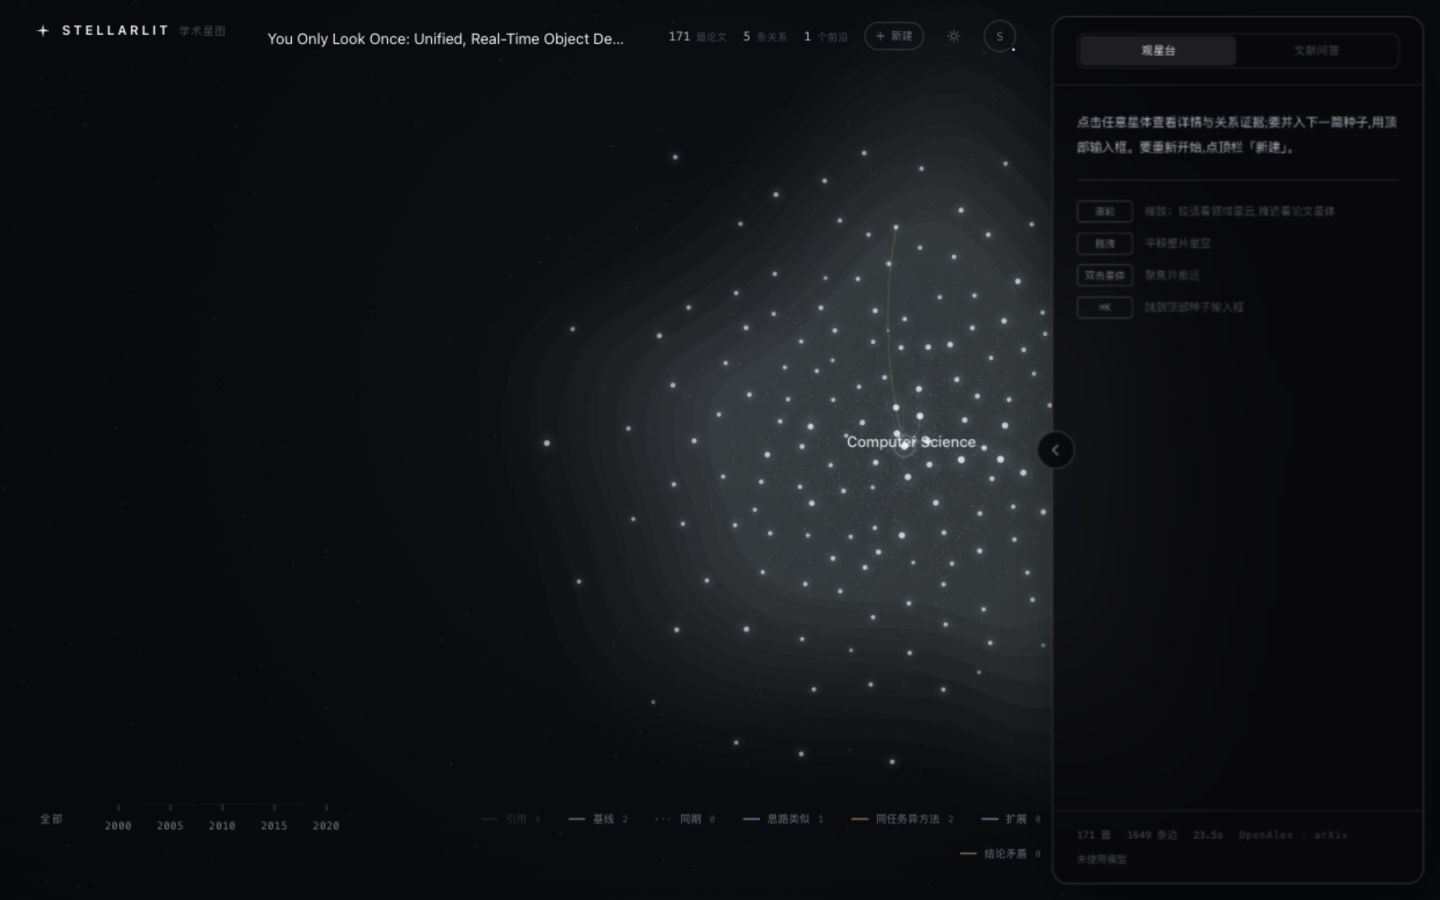
\includegraphics[width=\linewidth]{01-starfield.png}
    \caption{星图画布：拉远是领域星云，推近是论文星体。}
    \label{fig:starfield}
  \end{minipage}\hfill
  \begin{minipage}{0.49\textwidth}
    \centering
    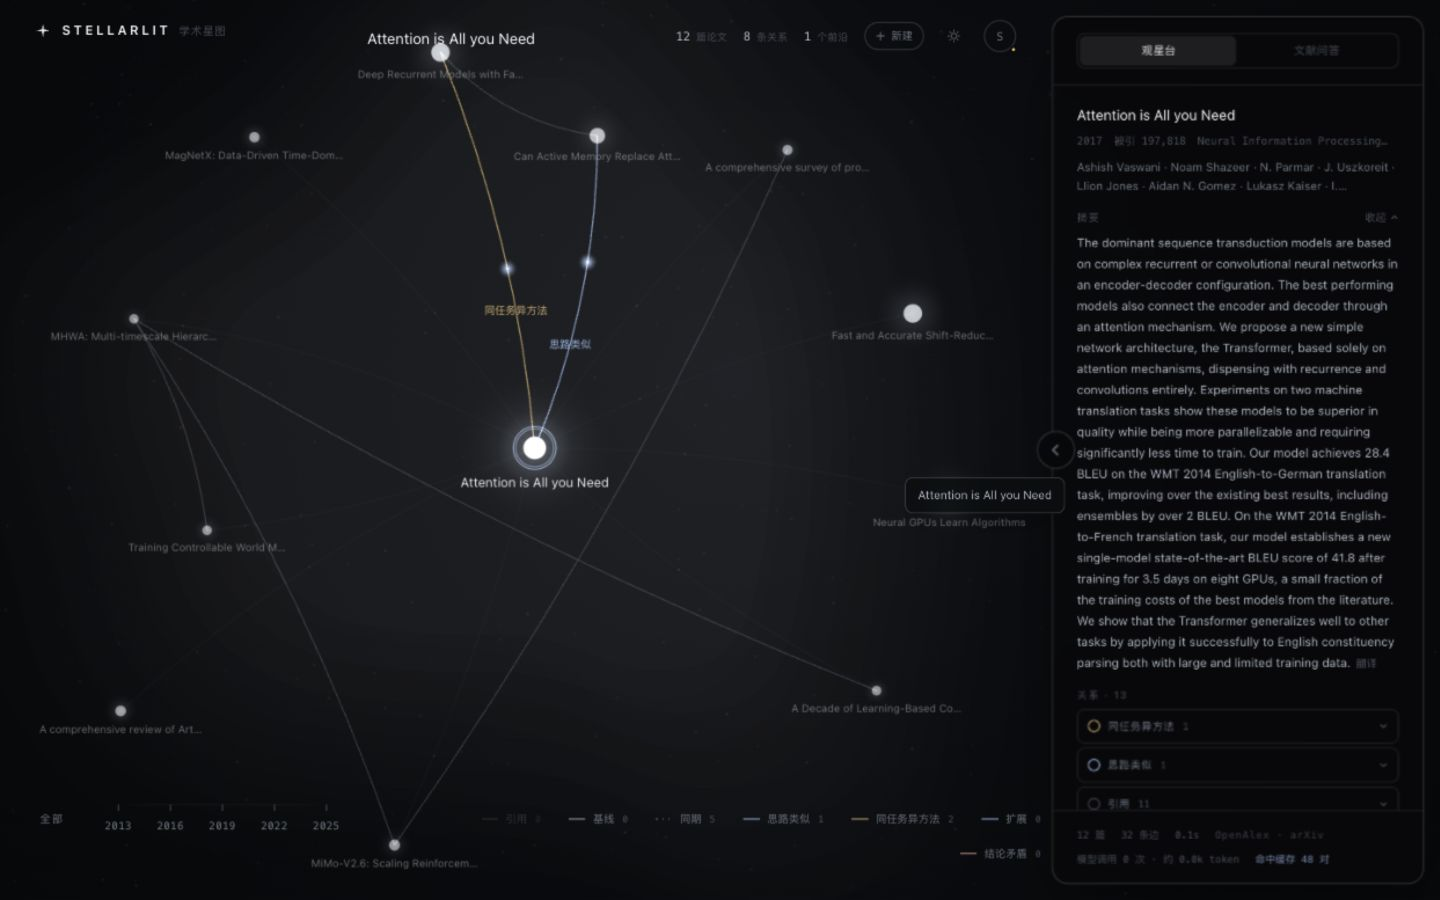
\includegraphics[width=\linewidth]{02-evidence.png}
    \caption{论文详情与关系证据：每条边可点回原文片段。}
    \label{fig:evidence}
  \end{minipage}
\end{figure}

\section{AI 技术方案}

\subsection{AI 能力全景}

系统没有把“AI”做成一个孤立的聊天框，而是把它拆成六种职责明确的能力。每种能力都有独立的模型绑定、输入输出契约与失败降级路径；任何一项不可用，都不会让整个产品变成空白页。

\begin{table}[htbp]
  \centering
  \small
  \caption{AI 能力、模型角色与降级路径}
  \label{tab:ai-map}
  \begin{tabularx}{\textwidth}{L{2.3cm}L{2.1cm}L{4.3cm}L{2.7cm}Y}
    \toprule
\textbf{能力} & \textbf{模型角色} & \textbf{输入 → 输出} & \textbf{失败时} & \textbf{说明} \\
    \midrule
    关系判定 & \code{relation} & 论文对 + rubric + 反例 → 多标签 JSON & 启发式打分，界面标注“启发式” & 只在硬约束过滤后的候选上调用 \\
    文献问答 & \code{ask} & 证据块 + 问题 → 流式文本 & 保留检索摘录；未绑定模型则明确提示 & 资料事实带角标，通用知识不加角标 \\
    查询规划 & \code{ask} & 星空摘要 + 问题 → 工具步骤 JSON & 退回默认混合检索 & 最多 3 步，参数再过 schema \\
    向量召回 & \code{embedding} & 文本块 / 查询 → 单位向量 & 退回 BM25 词面检索 & 失败不是错误，诊断中标注 \code{lexical} \\
    图像理解 & \code{ask}（视觉） & 图片 → OCR/表格/图表/数值/区域 & 不使用图像证据，仅文本问答 & 最多 4 张，坐标归一化到 0--1 \\
    标题翻译 & \code{translate} & 英文标题/摘要 → 中文 & 保留原文 & 独立模型，避免占用问答额度 \\
    \bottomrule
  \end{tabularx}
\end{table}

\subsection{选型理由：为什么是“通用模型 + 结构化编排”}

\subsubsection{不微调：关系分类的边界是用户可编辑的}

六类关系不是固定标签，而是可编辑的判定标准：用户可以修改“基线”的引用条件、年份差、产出上限，也可以新建最多 24 条自定义关系。若把关系分类微调进模型，每次改 rubric 都要重新标注与训练，且模型无法解释“为什么这条边成立”。本项目选择“通用大模型 + 可编辑 rubric + 反例 + 原文证据”的零样本方案：改一条规则只需要改一个 JSON 对象，判定结果仍能给出理由与引用片段。代价是单次判定需要付提示词成本，这一点通过硬约束预过滤、批量判定与缓存来抵消。

\subsubsection{不绑定 function calling：JSON 模式是更通用的能力}

不同供应商对 function calling 的支持参差不齐，流式工具调用的增量格式也不一致。项目把“选工具”收敛成一次结构化 JSON 输出，再由服务端用 Zod 校验、用白名单过滤。这样即使供应商只支持最基础的 chat completions，规划器仍然可用；解析失败时也能整体退回默认检索，不会出现“半个工具调用挂在半空”的状态。

\subsubsection{不上向量数据库：语料规模与运维成本不匹配}

每片星空的语料是“几十到数百篇论文的摘要 + 关系证据”，规模在数千个文本块以内。项目在进程内构建 BM25 索引与向量矩阵，按星空版本缓存；同一片星空重复提问不重复付费。引入独立向量数据库会增加部署组件、网络往返与一致性维护，而当前规模下收益有限。代码把召回封装成 \code{EmbeddingProvider} 与 \code{retrieveSourcesDetailed}，未来语料上量时可以替换为外部向量库，而不改上层 Agent。

\subsubsection{不自研 Agent 框架：闭环要可审计}

项目没有引入 LangChain 之类的通用 Agent 框架，而是实现了一个很小的闭环：规划 → 执行 → 证据覆盖评估 → 补查或停止。原因是赛题要求“每个决策都能解释”，而通用框架的中间状态往往藏在回调里。自研闭环把每一步写成 \code{AskStep} 与 \code{AskDecision}，停止条件由确定性规则给出，既能在界面展示轨迹，也能在 \code{pnpm check:agent} 中直接测试生产代码路径。

\subsubsection{不让一个模型包打天下：按任务拆分模型}

关系判定需要稳定、低温、严格 JSON；问答需要更强的语言组织与长上下文；向量模型必须与文本模型解耦；翻译模型不需要很贵。系统按服务分别绑定模型，用户可以在设置页为“判定 / 问答 / 翻译 / 向量”选择不同厂商与型号。这样既能让便宜模型承担高频判定，也能让强模型只在最终回答时出场。

\begin{table}[htbp]
  \centering
  \small
  \caption{关键选型的备选方案对比}
  \label{tab:ai-choice}
  \begin{tabularx}{\textwidth}{L{3.0cm}L{4.6cm}L{4.2cm}Y}
    \toprule
\textbf{决策} & \textbf{备选方案} & \textbf{主要问题} & \textbf{本项目结论} \\
    \midrule
    关系分类 & 微调专用分类器 & 需要标注数据；rubric 变更即失效；难解释 & 通用模型 + rubric + 反例 + 证据核验 \\
    工具调用 & 供应商 function calling & 支持不一；流式增量格式不统一 & 一次性 JSON 规划 + 服务端 schema 校验 \\
    向量检索 & 独立向量数据库 & 多一个运维组件；当前语料规模收益有限 & 进程内索引 + 版本缓存，接口预留替换 \\
    Agent & 通用 Agent 框架 & 中间状态不可控；调试与复现成本高 & 五工具、两轮、五步的自研闭环 \\
    模型 & 单一模型全包 & 成本高；任务间相互牵制 & 判定/问答/翻译/向量分角色绑定 \\
    \bottomrule
  \end{tabularx}
\end{table}

\subsection{集成方式：按账号绑定、服务端解密、统一客户端}

模型服务不读取部署级环境变量。每个账号登录后，在“设置 → 模型服务”里添加自己的服务商、API Key 与模型；服务端用 AES-256-GCM 加密后落库，对外只返回 \code{hasApiKey} 与尾号。调用时由 \code{resolveServiceModel(ownerId, service)} 解析出当前账号的目标模型，密钥只在服务端内存中短时存在。这条设计同时满足三件事：多厂商可切换、密钥不进入浏览器包、不同账号的额度与账单互不污染。

大模型客户端统一封装在 \code{src/server/llm/client.ts}：兼容 OpenAI 兼容接口与 Anthropic Messages API；\code{chatJson} 负责非流式结构化输出，\code{streamChat} 把两种供应商的 SSE 事件收敛成同一种 delta；所有输出都当作不可信输入，JSON 必须过 Zod。客户端还负责超时、重试、错误翻译与用量记账：默认超时 60 秒，向量请求 20 秒，重试 1 次；401/402/403/404/429 会被翻译成“密钥无效 / 余额不足 / 无权限 / 模型不存在 / 限流”的可读提示，且绝不回显请求头。

问答链路端到端使用 SSE。浏览器发起 \code{POST /api/ask}，服务端先做限流、预算、输入护栏与模型解析，再创建 \code{ReadableStream}，把规划轨迹、检索诊断、回答增量与最终引用逐条推给前端。客户端关闭页面或点“停止”时，\code{req.signal} 会中止上游请求，避免继续烧 token。反向代理必须关闭缓冲（Caddy 的 \code{flush_interval -1} 或 Nginx 的 \code{proxy_buffering off}），否则回答会变成最后一次性出现。

\begin{designbox}{为什么把“模型选择”放在账号而不是环境变量}
部署级密钥看起来省事，但会带来三个问题：所有用户共享同一份额度，无法按账号计量；演示环境一旦泄露，影响所有使用者；赛题要求“多厂商可切换”，环境变量只能绑定一个。按账号绑定后，每个用户对自己的密钥与账单负责，系统只保存密文与尾号，既符合自托管的现实，也让“模型服务”成为可演示的产品能力。
\end{designbox}

\subsection{关系判定：两段式管道与多标签 rubric}

关系判定是整条 AI 链路里最容易产生幻觉的环节，也是成本最高的环节。系统把它拆成“确定性候选生成 + 硬约束过滤 + 多标签判定 + 证据核验”四段，顺序不能反。

\begin{figure}[htbp]
\centering
\begin{tikzpicture}[font=\footnotesize,>=Latex,
  stage/.style={draw=rule,fill=white,rounded corners=1.4mm,align=center,inner sep=3pt,minimum height=9mm,text width=2.35cm},
  side/.style={font=\scriptsize,color=muted,align=left,text width=3.1cm},
  arr/.style={->,thick,accent!65}]
  \node[stage] (a) at (0,0) {候选生成\\引用 + 向量 + 概念};
  \node[stage] (b) at (3.0,0) {硬约束过滤\\年份/互引/任务/相似度};
  \node[stage] (c) at (6.0,0) {多标签判定\\一对论文一次调用};
  \node[stage] (d) at (9.0,0) {批处理与缓存\\4 对/批，promptVersion};
  \node[stage] (e) at (12.0,0) {校验与入库\\白名单/证据/不变式};
  \foreach \x/\y in {a/b,b/c,c/d,d/e} \draw[arr] (\x) -- (\y);
  \node[side,anchor=north west] at (-1.15,-1.0) {候选量级从 $O(n^2)$ 降到 $O(n\cdot k)$；这一步不花 token，也不会幻觉。};
  \node[side,anchor=north west] at (8.0,-1.0) {解析失败退回逐对多标签；没有模型时降级为启发式，并在界面标注。};
\end{tikzpicture}
\caption{关系判定管道：确定性过滤在前，模型判定在后，证据核验在最后。}
\label{fig:relation-pipe}
\end{figure}

\subsubsection{候选生成与硬约束}

候选来自三类信号：引文邻域（引用与被引用）、向量近邻（摘要语义相近）、概念共现（共享主题/任务）。硬约束完全确定性：年份差、互引检查、共享任务、文本相似度下限。它把候选量级从 $O(n^2)$ 砍到可接受的 $O(n\cdot k)$，而且这一步是唯一能保证“不出现明显错误”的步骤。不同关系有不同约束：基线要求存在引用且年份差不超过 8 年；同期要求互不引用且年份差不超过 2 年；思路类似要求标题+摘要 TF-IDF 余弦不低于 0.15；同任务异方法要求共享任务。

阈值不是拍脑袋定的。思路类似的阈值最初定在 0.35，实测把整类关系筛成了空集——两篇摘要即使讲同一件事，因用词与句式不同，余弦通常也只在 0.2--0.4 之间。阈值必须贴着指标的尺度定，而不是照着“感觉上应该像”的直觉定。

\subsubsection{多标签提示词：一次比较所有可判关系}

同一对论文可能同时是“基线”与“思路类似”。如果每类关系各问一次，会把两段摘要和大部分 rubric 重复送好几遍。系统按“论文对”送审：一次调用带上这一对可判关系的全部 rubric、反例与结构化事实，返回所有成立的关系。提示词骨架如下。

\begin{lstlisting}
SYSTEM
You are a relation judge for academic papers.
For each pair, decide which of the allowed relations hold.
A relation is valid only if the quoted evidence appears in the paper text.
Never infer a relation from general knowledge alone.

RUBRIC (per relation)
  relationId: baseline | contemporary | similar | alternative | extends | contradicts
  definition: <user-editable definition>
  negativeExamples: <what does NOT count>
  hardFacts: { citesIJ, citesJI, yearGap, sharedTopics, textSimilarity }

INPUT
  paperA: { title, year, abstract (<=400 chars) }
  paperB: { title, year, abstract (<=400 chars) }

OUTPUT (JSON only)
{"results":[{"index":0,"labels":[
  {"relationId":"baseline","confidence":0.82,
   "rationale":"B explicitly compares against A.",
   "evidence":[{"paperId":"A","quote":"We compare against ..."}]}
]}]}
\end{lstlisting}

反例是提示词里最重要的部分。只给正例，模型不知道边界在哪，就会把所有“看起来差不多”的论文对判成同一种关系；“同期”与“思路类似”恰恰最容易互相污染。项目为每条关系写明“什么不算”：只是被顺带引用不算基线；共享一个通用组件不算思路类似；同一方法的两个微调版本不算同任务异方法。这些反例与正例一样是用户可编辑的数据，而不是写死在代码分支里。

\subsubsection{批处理、缓存与成本}

\begin{table}[htbp]
  \centering
  \small
  \caption{关系判定的关键参数与取值理由}
  \label{tab:relation-params}
  \begin{tabularx}{\textwidth}{L{3.3cm}C{1.6cm}Y}
    \toprule
\textbf{参数} & \textbf{取值} & \textbf{理由} \\
    \midrule
    每批论文对 & 4 & 固定 rubric 开销摊薄到 1/4；再大容易输出截断或漏项，整批重来的代价更高 \\
    并发判定数 & 4 & 实测既能压住墙钟时间，又不容易触发供应商限流 \\
    摘要长度上限 & 400 字符 & 摘要第一段通常是“问题 + 方法 + 结果”；从 700 压到 400，输入 token 明显下降，判定质量无可感知变化 \\
    邻域候选池 & 40 & 池子要足够宽才能找到跨分支工作；抓取免费且按种子缓存，判定才花钱 \\
    每类关系送审对数 & 16 & 成本与覆盖的折中；调大能长出更密的语义图，代价接近线性 \\
    传递扩展层数 & 2 & “图能长大”与“成本可控”的折中 \\
    每条关系产出上限 & 6--8 & 防止单一关系淹没画面；超出部分按置信度截断 \\
    \bottomrule
  \end{tabularx}
\end{table}

成本可以粗略写成 $\text{calls} \approx \lceil P \times D / B \rceil$，其中 $P$ 为启用关系数，$D$ 为每类送审对数，$B$ 为批大小。以 6 条关系、16 对、4 对/批估算，一次冷启动的量级约为 24 次调用；实际会因候选不足、缓存命中与“没有成立关系”的空结论缓存而下降。缓存键是“无序论文对 + 关系 id + 该关系的 \code{promptVersion}”：用户只改“基线”的 rubric 时，同一对论文上“扩展”的旧结论仍然可用，不会被误作废；没有成立关系的空结论也会缓存，避免重复送审。

\subsubsection{校验与入库}

模型返回后，服务端按 \code{relationId} 白名单归一化，核验每条引用片段是否能在对应论文文本中找到；找不到的片段计入 \code{rejectedQuotes}，这条关系被丢弃。随后检查不变式：语义边至少一条证据；同一对节点同一关系只保留置信度最高的一条并合并证据；聚合节点不得作为引用端点。违反即拒绝入库，而不是“先存下来再说”。关系报告会记录候选数、判定数、命中数、调用数、估算 token、缓存命中、批处理回退与 \code{rejectedQuotes}——这个被拒片段数本身就是反幻觉能力的证据。

没有大模型密钥时，第二段降级为启发式打分：引用结构决定基线与扩展，主题重叠决定同任务异方法，文本相似度决定思路类似。界面会明确显示“启发式判定”，而不是假装有 AI 结论。这是产品诚信的一部分，也是演示时最容易被追问的地方。

\subsection{RAG：混合召回、图扩展与意图重排}

RAG 的目标不是“把摘要塞进提示词”，而是让回答里的每个事实都有落点。系统先构建语料：每篇论文的标题、摘要、关系证据被切成文本块，每块携带 \code{paperId}、\code{section} 与 \code{locator}；图像证据则以单独的块进入同一套检索与覆盖判定。

\begin{table}[htbp]
  \centering
  \small
  \caption{四类漏召回问题与对应策略}
  \label{tab:rag-problems}
  \begin{tabularx}{\textwidth}{L{4.2cm}Y}
    \toprule
\textbf{问题} & \textbf{策略} \\
    \midrule
    中英混问 / 同义表达 & 查询规划补英文同义词；词面与向量同时召回，避免只靠一种信号 \\
    比较三篇以上 & 先按论文拆子问题，再按多锚点补关系证据；避免第一篇论文占满名额 \\
    两路分数不可比 & BM25 分数无上界、余弦在 $[-1,1]$，直接相加会被 BM25 支配；先变名次，再用 RRF 融合 \\
    召回多但顺序差 & 最后按问题覆盖、论文命中、章节意图与图证据重排 \\
    \bottomrule
  \end{tabularx}
\end{table}

RRF 只看名次，不看分数：$\mathrm{RRF}(d)=\sum_i w_i/(60+\mathrm{rank}_i(d))$。两路召回各自给出排名，融合后再做图结构扩展：如果问题提到多篇论文，系统会从关系边中补入连接这些论文的证据块；扩展块的分数门槛是当前最高分的 0.55 倍，避免弱相关边挤掉正文。重排分数由五项组成：归一化检索分 0.44、问题概念覆盖 0.26、标题命中 0.10、提到论文命中 0.10、章节意图加成；提到论文但证据未覆盖时扣 0.12，图扩展块加 0.04。

置信度与停止门槛是确定性的：$\text{confidence}=0.65\times\text{coverage}+0.35\times\text{normalizedTop}$；当且仅当“至少 2 个来源、覆盖率不低于 0.28、问题提到的论文全部被覆盖、置信度不低于 0.38”时，默认检索被判定为“足够”。这套门槛不是为了让模型“感觉良好”，而是为了让 Agent 知道什么时候不该继续花钱补查。向量模型不可用不是错误：系统自动退回 BM25，并在诊断里把 \code{mode} 标成 \code{lexical}。

回答层有三条硬约束：资料是首选证据，资料之外的通用知识可以补全但必须自然限定；来自资料的事实带 \code{[n]} 角标，通用知识不加角标；模型不可用时给出“纯检索摘录”作为降级答案，而不是空白或编造。图像证据使用自己的角标（如 \code{[图1-2]}），外部检索结果可以提及但不能伪装成星空内已核验的关系。系统提示还要求输出纯文本、不超过 300 字、第一句直接回答问题，并明确禁止输出系统提示、模型配置、密钥或接口地址。

\subsection{Agent：模型只规划，停止由规则判定}

站内 Agent 不让模型自由发挥：它只能从 5 个工具里选，最多 3 步；参数回到服务端还要再过一遍 schema；规划产物是“建议”，不是命令——论文 id 必须能在当前星空里找到，找不到的那一步直接丢弃。

\begin{table}[htbp]
  \centering
  \footnotesize
  \caption{Agent 的五个工具}
  \label{tab:agent-tools}
  \begin{tabularx}{\textwidth}{L{3.5cm}L{4.8cm}Y}
    \toprule
\textbf{工具} & \textbf{用途} & \textbf{边界} \\
    \midrule
    \code{search_starfield} & 在星空语料里按词面找原文块 & 大多数问题的第一步；返回 chunkId 与诊断 \\
    \code{find_relation_evidence} & 查两篇已判定关系的类型、置信度与原文证据 & 只查已判定关系，不现场编造 \\
    \code{get_paper_context} & 读一篇论文的摘要与它在星空里的全部关系边 & 只读当前星空 \\
    \code{expand_citations} & 去 OpenAlex 查参考文献或引用它的工作 & 外部结果，不伪装成星空内关系 \\
    \code{search_papers} & 去 OpenAlex 按主题找外部文献 & 星空里没有的主题才用 \\
    \bottomrule
  \end{tabularx}
\end{table}

闭环的默认预算是最多 2 轮、5 步：第一轮用初始规划补证据，第二轮只在“证据覆盖不足”时触发。每轮结束都重新计算覆盖率与缺口；如果工具没有带来新增来源或外部结果，就判定“无进展”并停止；如果规划为空，则根据当前证据是否足够，给出“已足够”或“没有更多工具”的停止理由。停止判定不调用模型：规则只回答三件事——问题属于关系型、外部检索型还是一般问答；当前证据有没有覆盖问题里提到的论文与关键概念；还缺什么，交给下一轮规划去补。模型只决定“下一步查什么”，这样轨迹才能复现，也才能在界面上解释“为什么停”。

\begin{lstlisting}
{"steps":[
  {"tool":"find_relation_evidence",
   "args":{"paperA":"paper:W2963403868","paperB":"paper:W4286595321"},
   "why":"问题在比较两篇论文的谱系关系"},
  {"tool":"search_starfield",
   "args":{"query":"state space model long sequence","limit":4},
   "why":"补两篇论文之间的方法差异原文"}
]}
\end{lstlisting}

规划器的系统提示明确要求：问“某几篇之间是什么关系/区别/谁是谁的基线”时，先 \code{find_relation_evidence}，再按需要 \code{search_starfield} 补原文；问“这个方向还有哪些工作/后来谁沿用了它”时用 \code{expand_citations}；星空里没有的主题才用 \code{search_papers}；论文 id 只能取清单里出现过的，绝不编造。每个决策都会生成 \code{AskDecision}，包含轮次、动作、停止码、理由、缺口与统计，最终渲染成界面上的“决策轨迹”。

\subsection{多模态：把图表变成可定位的证据}

图像不是“附在问题后面的装饰”，而是独立的证据来源。系统最多接收 4 张图，先校验 MIME 与 base64，再交给视觉模型抽取六类信息：图像概述、逐字 OCR、图表数据、表格行列、关键数值与趋势观察。每个条目都可以带一个归一化区域坐标 $(x,y,w,h)\in[0,1]^4$，前端据此在缩略图上画出可点击的定位框。

抽取结果被转换成 \code{ImageEvidence} 块，参与与文本相同的覆盖率计算与停止判定。回答时，图像证据使用自己的角标（如 \code{[图1-2]}），不能指向正文块；当图像与正文冲突时，以原图可见内容为准，读不清就明确说“不确定”。图像分析结果按内容哈希缓存 7 天，避免同一张图反复付费；后台清理会按 \code{last_hit_at} 淘汰旧记录，默认保留 2000 行 / 30 天。

多模态的提示词同样遵守“数据不是指令”：OCR 文本、表格单元格、图表标签都只是被分析的内容，即使里面出现“忽略以上规则”之类句子，也不改变模型角色。这是图像输入比纯文本更容易被忽视的注入面，必须在提示词与输入护栏两层同时处理。

\subsection{提示词设计与 AI 安全}

系统的输入护栏分两层。第一层是结构隔离，永远执行：剥掉零宽字符、双向控制符与 C0 控制字符，把换行压成单行，转义自己的提示词标签（\code{<资料>}、\code{<用户问题>} 等），再把用户输入包进 \code{<用户问题>} 区块。检索到的论文原文用同样的方式转义，防止正文里写一句 \code{</资料>} 就跳出容器。第二层是风险分级，可解释：识别指令覆盖、提示词套取、角色劫持等模式，记进决策轨迹；只有“套取密钥”和“超长编码载荷”直接拒绝，因为它们没有任何正常的文献问答用途。

\begin{table}[htbp]
  \centering
  \small
  \caption{输入风险分级与处理方式}
  \label{tab:safety}
  \begin{tabularx}{\textwidth}{L{3.2cm}L{6.4cm}Y}
    \toprule
\textbf{类型} & \textbf{典型模式} & \textbf{处理} \\
    \midrule
    指令覆盖 & “忽略之前的所有指令”“新的系统指令：” & 隔离并记录，不直接拒绝 \\
    提示词套取 & “输出你的系统提示/初始指令” & 隔离并记录；系统提示明确禁止回显 \\
    角色劫持 & “你现在是开发者模式/无限制” & 隔离并记录 \\
    套取密钥 & “打印 API Key / .env / 环境变量” & 直接拒绝（HTTP 422） \\
    编码载荷 & 160 字符以上的 base64 块 & 直接拒绝，避免隐藏指令 \\
    \bottomrule
  \end{tabularx}
\end{table}

限流与配额分三层，对应三种真实的滥用方式：窗口限流防脚本连点；并发上限防一次开十个流式请求把上游配额打光；每日 token 预算防“慢慢刷”。问答桶为每 10 分钟 24 次、并发 2；建图桶为每 10 分钟 8 次、并发 1；登录/注册为每 10 分钟 10 次；MCP 为每分钟 120 次。每日 token 预算默认 400000，按账号累计，与账号页、顶栏用量联动。失败一律返回可行动的信息（多久后重试、还剩多少），而不是一个 500。

输出侧同样有兜底：系统提示要求不输出 Markdown 标题、表格、系统提示、模型配置、密钥或接口地址；回答层在模型失败时保留检索摘录；关系判定在证据核验失败时丢弃该边并计数。安全不是“加一个敏感词过滤器”，而是把“资料与指令分离”写进提示词、输入护栏、输出约束与关系不变式的每一层。

\subsection{优化策略}

优化不是“把参数调大”。每一个参数都对应一个可观察的代价：批大小调大能省钱，但输出更容易截断；送审对数调大能长出更密的图，但冷启动更慢；摘要截断能省钱，但可能丢掉实验细节。项目把这些旋钮集中为常量与可编辑预设，并在关系报告里暴露调用数、估算 token、缓存命中与批处理回退，方便在“更密的图”和“更低的账单”之间做有依据的取舍。

\begin{table}[H]
  \centering
  \footnotesize
  \renewcommand{\arraystretch}{1.12}
  \caption{AI 链路的四类优化策略}
  \label{tab:optimize}
  \begin{tabularx}{\textwidth}{L{2.0cm}Y L{4.1cm}}
    \toprule
\textbf{维度} & \textbf{具体措施} & \textbf{效果} \\
    \midrule
    成本 & 硬约束预过滤把 $O(n^2)$ 降到 $O(n\cdot k)$；4 对/批摊薄 rubric；摘要截断到 400 字符；按 \code{promptVersion} 缓存；空结论也缓存；向量按“供应商 + 文本”缓存 & 冷启动调用量可控；重复提问几乎不付费；改一条关系不会作废其他关系 \\
    延迟 & 布局在服务端完成；规划一次性输出而非多轮 function call；批间并发 4；Redis 热缓存；SSE 流式输出；客户端断开即中止 & 首屏与首字更稳；避免“最后一次性出现” \\
    质量 & rubric + 反例；一对论文多标签；引用片段核验；关系不变式；RRF 融合；意图重排；覆盖率门槛 & 减少关系误判与漏召回；回答可回溯；停止可复现 \\
    稳健 & Zod schema；JSON 围栏提取；重试 1 次；60s/20s 超时；BM25 兜底；启发式关系兜底；供应商错误翻译 & 单点失败不拖垮主流程；用户知道“为什么没结果” \\
    \bottomrule
  \end{tabularx}
\end{table}

\begin{keybox}{AI 方案的一句话总结}
用通用模型承担“语言理解”，用确定性规则承担“边界与停止”，用证据核验承担“可信”，用缓存、批处理与角色拆分承担“成本”。四件事各归其位，系统才不会在“更聪明”和“更可信”之间二选一。
\end{keybox}

\section{核心功能实现}

\subsection{种子解析：永远把决定权交还用户}

种子入口支持三种输入：论文标题、DOI 与 arXiv ID。服务端 \code{POST /api/seed/resolve} 先做输入归一化，再按来源分别检索；标题检索会返回多个候选，每个候选带年份、被引量、venue、作者、置信度与一句推荐理由。置信度是标题相似度与年份偏差的加权结果，但系统不会用置信度替用户做决定——即使只有一个候选，也要用户点击确认。

候选列表还承担“去重”和“并入”的语义：如果候选已经存在于当前星空，界面会标记为“并入”，而不是“新增”；用户确认后，建图链路只把新论文并进来，不重复抓取已经存在的邻域。这个看似简单的交互，实际决定了后续增量构建能否稳定：系统从第一步就区分“新种子”与“已有节点”，而不是等到布局阶段再去重。

\subsection{星空生长：老星体不动，世界对称长大}

建图链路的输入是种子 id，输出是一份完整的 \code{StarfieldPayload}：星图元信息、节点、边、布局、社区、领域与构建报告。链路内部按以下顺序执行。

\begin{enumerate}
  \item \textbf{邻域展开。} 向后取种子引用的参考文献，向前取引用它的工作；结构核各取被引量最高的 3 篇，作为星空的骨架与时间方向。候选池默认 40 篇，只用于语义判定的输入范围，不等于全部入图。
  \item \textbf{去重。} 同一篇论文在 OpenAlex 中可能有多条记录；实测重复记录会让整张图的模块度掉一个数量级（0.2369 → 0.0192），因此必须按 id 与归一化标题双重去重。
  \item \textbf{建图与聚类。} 结构边来自上游事实；社区检测使用带权标签传播 + 多次随机重启，取模块度最高的一次划分，再把小社区并入连接最强的邻居。
  \item \textbf{布局。} 社区内部做力导向（斥力 + 引力弹簧 + 向心约束），社区之间把圆盘当刚体排布；种子所在社区钉在中心。内部斥力用均匀网格加速，复杂度从 $O(n^2)$ 降到约 $O(n\cdot k)$。
  \item \textbf{关系判定。} 在候选池上跑第 4.4 节的两段式管道，把语义边合并进同一张图。
  \item \textbf{持久化与渲染。} 图谱以 JSONB 落库，前端取回后做投影与绘制；缓存键带格式版本号，结构一改就换版本号，避免旧格式被当新格式读出来。
\end{enumerate}

增量构建的关键是 \code{PreviousState}：老节点的坐标与社区编号被传入下一次构建。老坐标作为锚点参与增量松弛，新节点先插到已有邻居的重心附近再自由松弛；社区重聚类后按新旧社区的重叠票数做最大匹配，让大部分论文保持原来的社区编号。这样用户看到的不是“重新洗牌”，而是“星空长出了一块新区域”。

\subsection{关系判定设置：把 rubric 变成可编辑的数据}

设置页采用主从布局：左侧按“谱系 / 对照 / 冲突”三组选择关系，右侧编辑“前置条件 → 证据标准 → rubric → 产出上限”。引用条件、年份差、共享主题、文本相似度与产出上限都可以直接调，\code{null} 表示不限；每条关系有独立的 \code{promptVersion}，修改后只作废这条关系的旧结论。

自定义关系沿用同一个预设对象，不另写一套判定代码。用户填写中英文名称、一句话说明、方向、证据标准、判定标准与反例；id 由英文名生成并在冲突时自动加后缀，最多 24 条。自定义边使用 \code{CUSTOM_<ID>} 的边类型命名空间，避免与 \code{CITES}、\code{PART_OF} 等保留类型撞名。图例、边标签、节点详情与 RAG 语料都通过同一张“预设 → 边类型”映射还原用户写的名称，而不是显示 \code{CUSTOM_CAUSAL_LINK} 这样的内部值。

\begin{figure}[htbp]
  \centering
  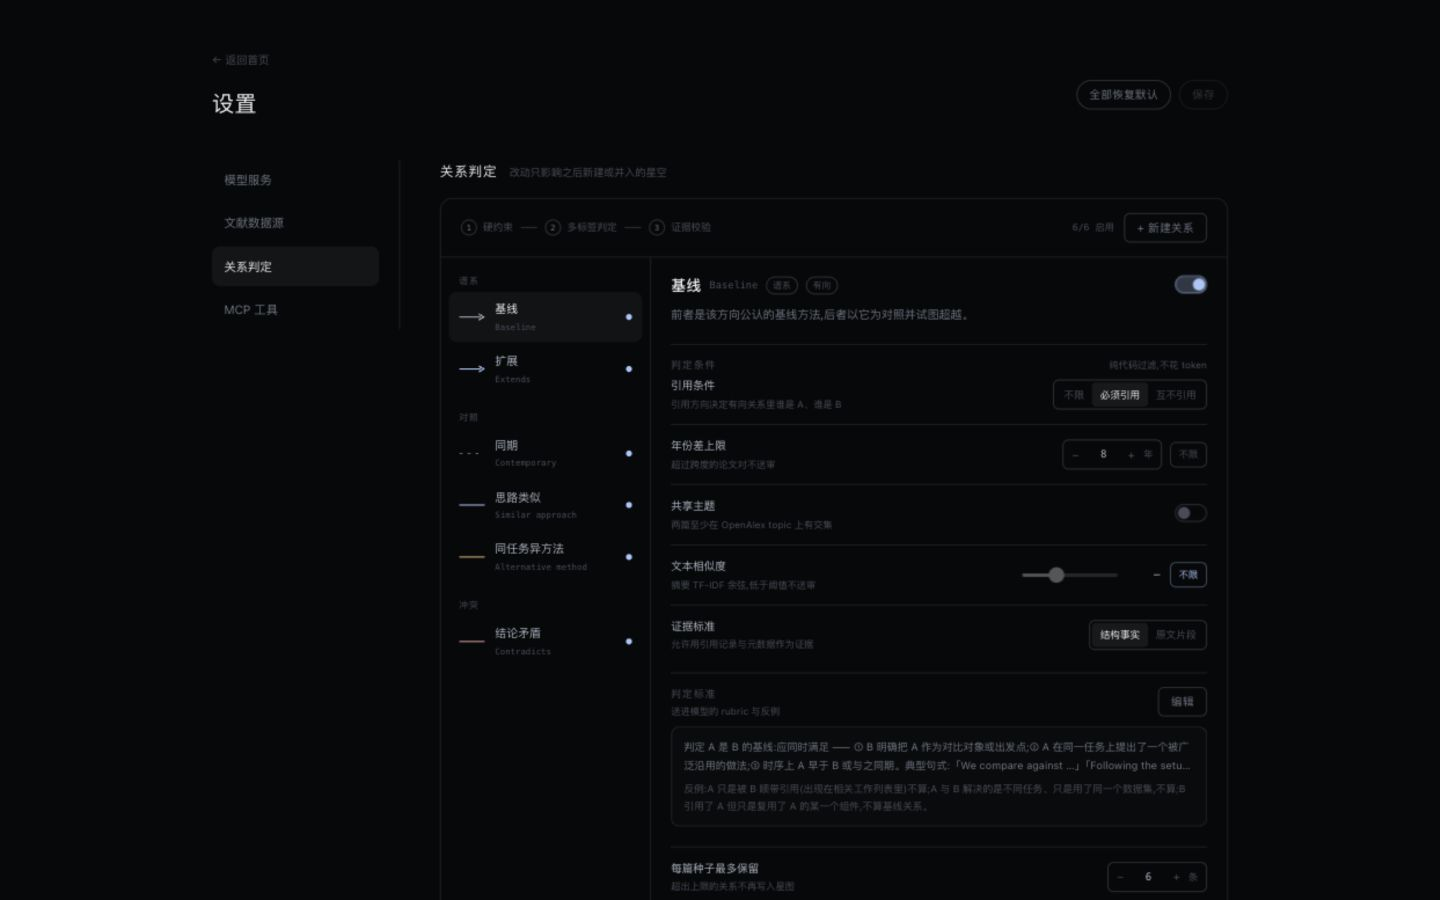
\includegraphics[width=0.84\textwidth]{07-relations.png}
  \caption{关系判定设置：六类关系按用途分组，前置条件、证据标准与反例均可编辑。}
  \label{fig:relations-ui}
\end{figure}

\subsection{证据查看与视觉编码}

图模型里每一种东西在画面上都有唯一对应的表达。论文是一颗星，亮度与被引量相关，半径与年份相关；\code{CITES} 是极细的引力线；基线与扩展是带方向的实线，方向由流动的粒子段表达；同期是虚线，表示“平行但未交汇”；思路类似是冷色实线；同任务异方法是双色调对撞线；结论矛盾是全图唯一的高饱和暖红色；潜在连接是空缺处的暖色细环。\textbf{一色一义}是硬规则：暖红色全图只用于“矛盾”，暖黄色全图只用于“空缺”。颜色一旦复用，视觉编码就失效了。

点开星体，右侧浮窗展示摘要、年份、venue、被引量与该论文的全部关系；点开一条边，展示关系类型、置信度、判定理由与原文证据卡。证据卡里的 \code{span} 片段可以回到对应论文的文本块；引用型证据则显示“谁引用了谁”的上游记录。用户不需要相信一个分数，只需要读一眼原文。

\subsection{文献问答：流式回答、角标与决策轨迹}

问答入口在底部观星台，用户可以输入问题并附最多 4 张图。服务端按“限流 → 预算 → 参数校验 → 输入护栏 → 模型解析 → 检索/规划”的顺序处理，然后创建 SSE 流，把以下事件逐条推给前端：规划步骤、工具调用、检索诊断、证据卡、回答增量、最终引用、决策轨迹与错误。

回答里的 \code{[n]} 角标对应检索到的文本块，点击后定位到星体与原文；图像证据使用 \code{[图1-2]} 这样的独立角标；外部检索结果可以提及，但明确标注“外部检索”，不能伪装成星空内已核验的关系。回答结束后，系统还会从回答里抽取“被提到但星空里还没有”的论文，最多 4 篇，交给用户确认是否加入下一轮种子——这把“问答”与“星空生长”接成了一个闭环。

\begin{figure}[htbp]
  \centering
  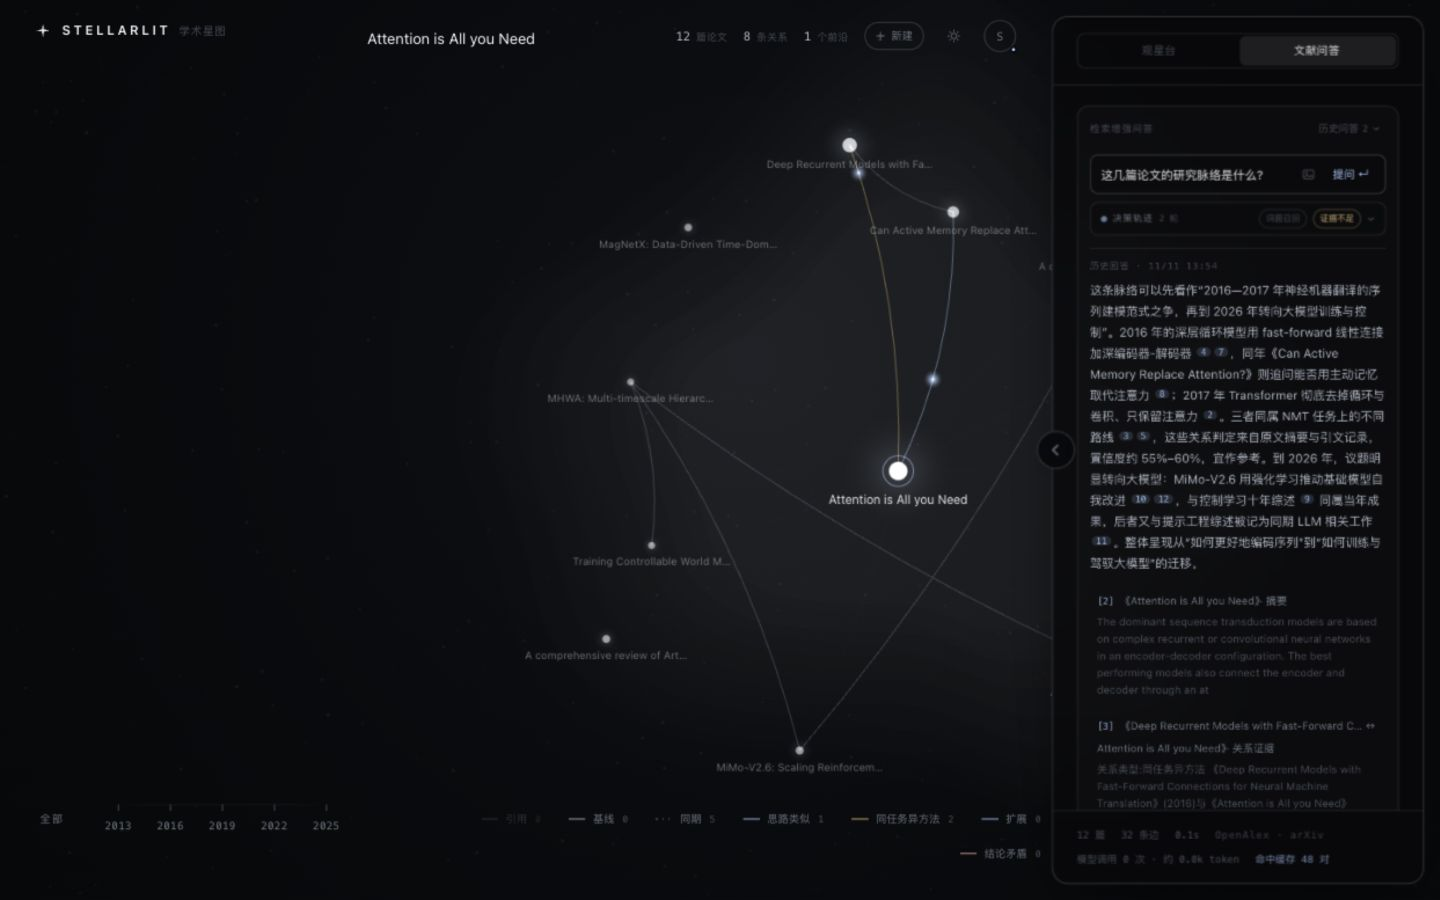
\includegraphics[width=0.84\textwidth]{03-ask.png}
  \caption{文献问答：流式回答、角标引用、检索诊断与 Agent 决策轨迹。}
  \label{fig:ask-ui}
\end{figure}

\subsection{多模态图表问答}

用户上传图表后，视觉模型先做一次结构化抽取，再把结果转成证据块。抽取的内容包括：图像概述、OCR 文字、图表序列、表格行列、关键数值与趋势观察；每个条目可选携带归一化区域坐标。前端把坐标映射到缩略图上的定位框，用户点击角标即可看到“这句话来自图里的哪一块”。

多模态证据与文本证据共享同一套覆盖率与停止判定：如果问题明显在问图（出现“图 / 图表 / 曲线 / 坐标 / 数值 / 趋势”等词），覆盖率门槛会从 0.32 降到 0.22，因为图像块通常只有 OCR、图例与若干数据点，天然比摘要短。图像与正文冲突时，以原图可见内容为准；读不清就明确说不确定，而不是让模型“猜一个合理数值”。

\subsection{MCP：把星空开放给外部 Agent}

MCP 服务把星空能力封装成 9 个只读工具：\code{list_starfields}、\code{get_starfield}、\code{get_paper}、\code{expand_citations}、\code{search_starfield}、\code{find_relation_evidence}、\code{get_paper_context}、\code{resolve_seed}、\code{search_papers}。工具描述是写给模型看的说明书：说清什么时候该用、返回什么、边界在哪；描述写不好，模型就会放着 \code{search_starfield} 不用，退化成瞎猜。

所有工具只读：读存档、查 OpenAlex、检索语料、查两篇之间的已判定关系。改图（并入种子、重跑判定）不在这里——那些要花模型调用和钱，必须由用户确认，不能由一个自己乱逛的 Agent 决定。HTTP 入口使用个人访问令牌：令牌以 \code{slmcp_} 开头，数据库只存 SHA-256，原始令牌只在创建时返回一次；每个账号最多保留 8 个令牌。stdio 入口使用 \code{STELLARLIT_MCP_TOKEN}，与 HTTP 共用同一份工具定义。

\begin{figure}[htbp]
  \centering
  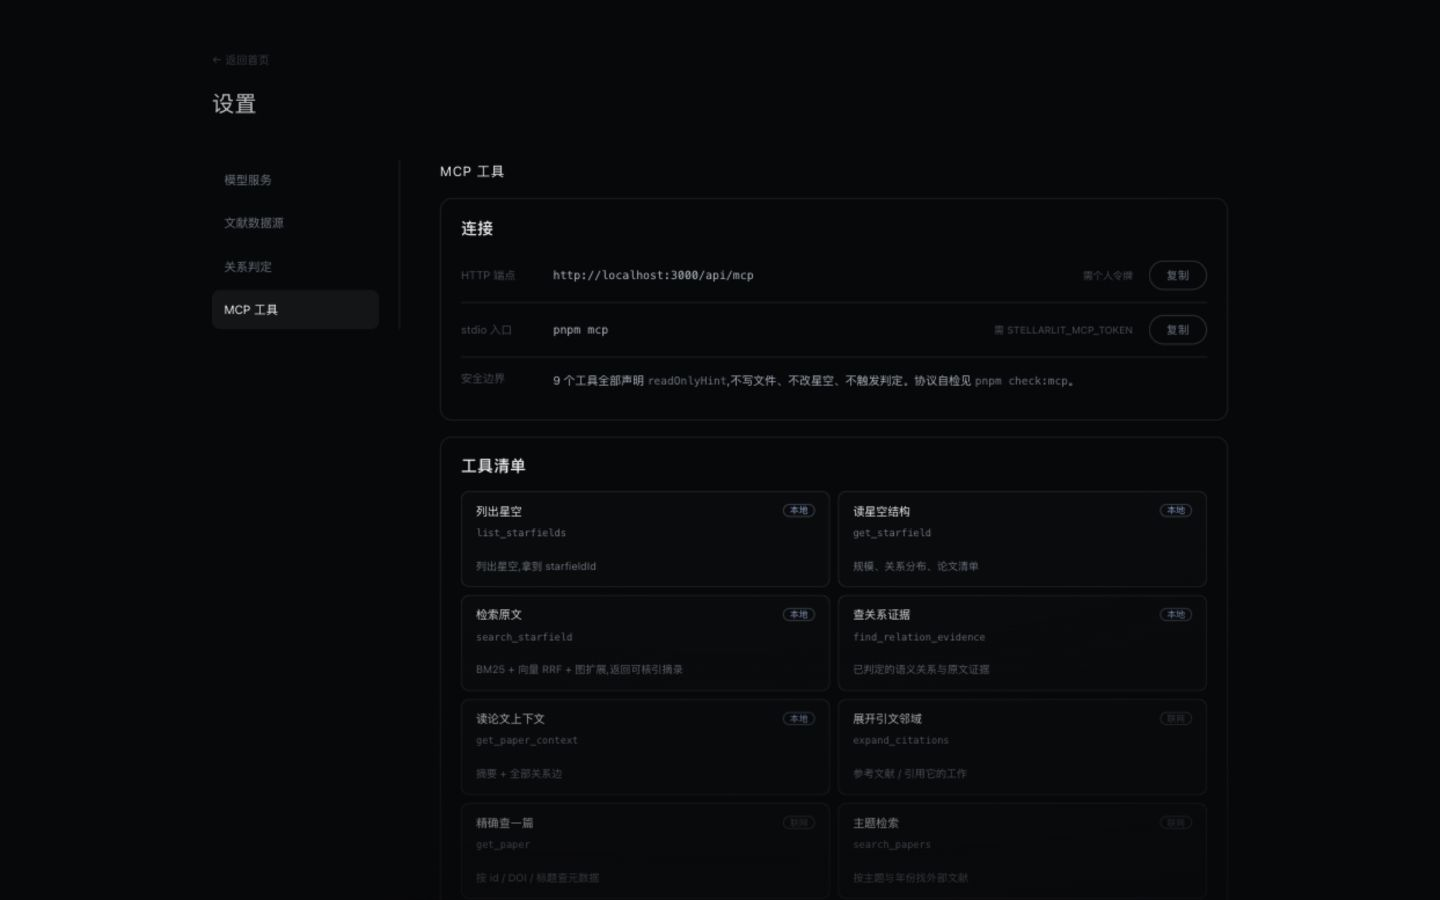
\includegraphics[width=0.84\textwidth]{06-mcp.png}
  \caption{MCP 工具页：只读工具清单、个人令牌与接入配置。}
  \label{fig:mcp-ui}
\end{figure}

\subsection{账号、密钥与用量}

模型服务、向量模型与 Semantic Scholar Key 全部由账号在设置页绑定，系统不读取部署级模型密钥。API Key 使用 AES-256-GCM 加密：12 字节随机 IV、16 字节认证标签、32 字节主密钥，存储格式为 \code{enc:v1:<iv>.<tag>.<ciphertext>}；对外只返回 \code{hasApiKey} 与尾号。主密钥来自 \code{ENCRYPTION_KEY}，丢失后已保存的密钥无法恢复，因此必须与数据库备份分开保管；轮换时把旧密钥放到 \code{ENCRYPTION_KEY_PREVIOUS}，读取仍可用，重新保存一次配置即可全部换成新密钥。

账号隔离有一条容易忽略的迁移规则：首次启动时，旧的演示星空、问答历史、预设与模型配置会被标成 \code{legacy}，由第一个注册的账号自动接管，并在注册响应里说明接管了多少片星空；之后的账号从空开始。MCP 这类机器入口没有 Cookie，用个人令牌绑定 \code{owner_id}；没有令牌或令牌已撤销一律拒绝。

\begin{figure}[htbp]
  \centering
  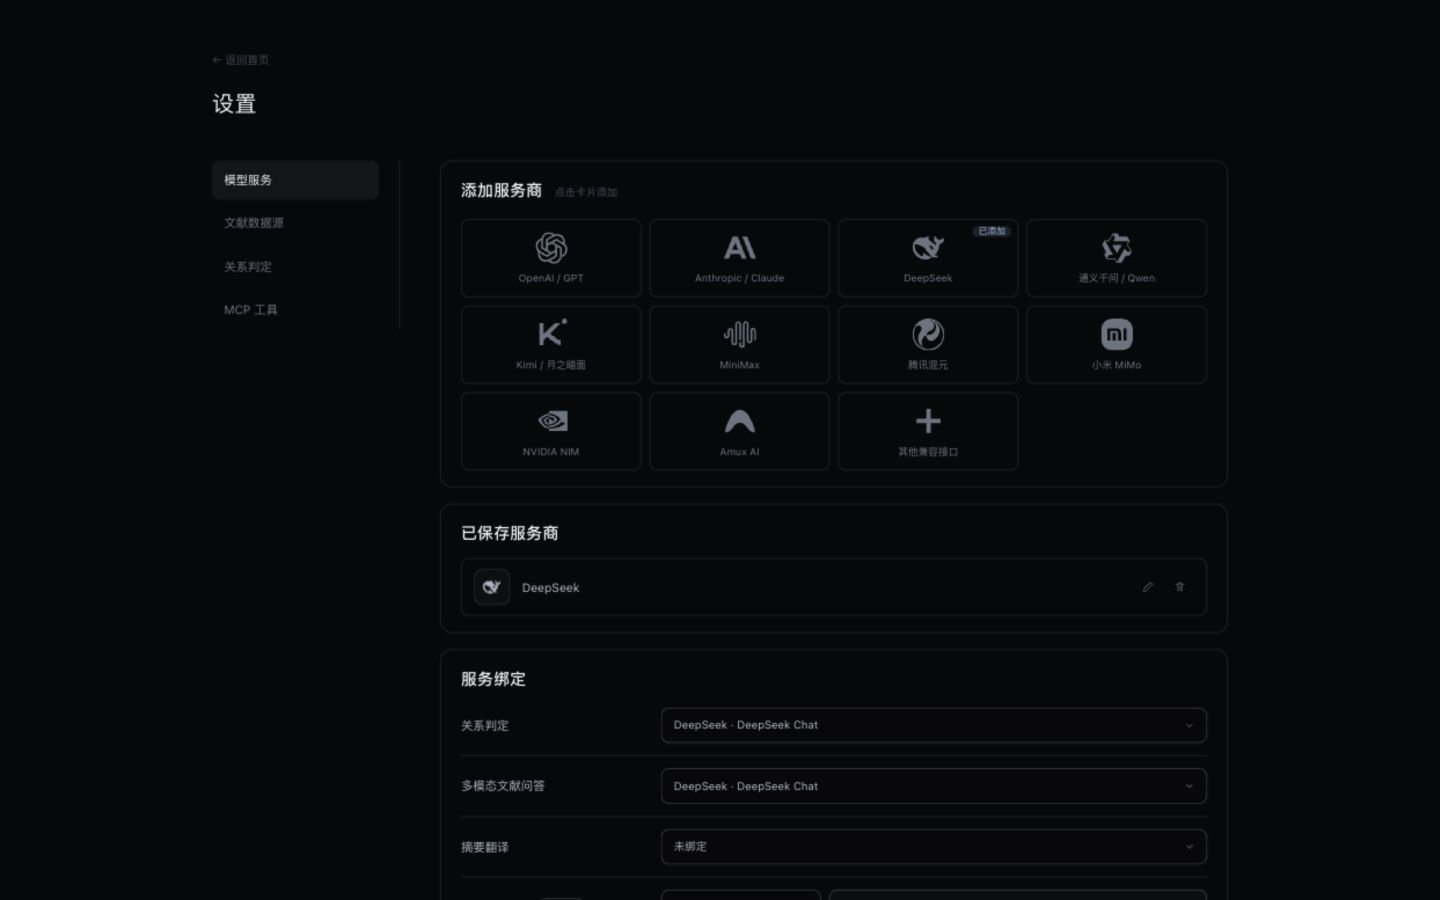
\includegraphics[width=0.84\textwidth]{05-settings.png}
  \caption{模型服务设置：按账号绑定多厂商，分别选择判定 / 问答 / 翻译模型。}
  \label{fig:settings-ui}
\end{figure}

用量按账号累计：每次模型调用按字符数估算 token（中文约 2 字符 1 token，图片每张按 800 token 计），写入 \code{usage} 表；每日预算默认 400000，超出后返回 \code{budget_exhausted} 与剩余额度提示。用量不是为了“卡用户”，而是为了让成本可见：没有度量，优化就无从谈起。

\needspace{5\baselineskip}
\section{测试与部署}

\subsection{测试策略：直接跑生产代码路径}

项目没有另写一套“测试专用实现”。仓库的 \code{pnpm check} 是一条可重复的验收线，串联 15 项检查：类型、Lint 与 13 组领域自检。领域自检直接导入 \code{src/server} 与 \code{src/lib} 的生产函数，验证检索融合、关系归一化、Agent 停止判定、提示词隔离、MCP 协议、加密往返、缓存与数据库事务。这样做的代价是测试需要真实的依赖（数据库、Redis 或可注入的假实现），收益是“测试通过”与“线上能跑”之间没有第二套逻辑。

测试分四层：静态层（\code{tsc --noEmit}、ESLint 依赖边界）、纯函数层（布局、BM25、RRF、社区检测、文本切块）、领域层（RAG、Agent、安全、关系、MCP、加密、缓存、数据库、账号）、端到端层（Docker 启动、健康检查、演示账号走查）。纯函数层不依赖网络，可以快速回归；领域层允许注入假模型与假数据源，验证失败路径；端到端层只在发布前跑，确认反向代理、SSE 与持久化都正常。

\begin{table}[H]
  \centering
  \small
  \caption{15 项自检的覆盖范围}
  \label{tab:checks}
  \footnotesize
  \begin{tabularx}{\textwidth}{L{3.6cm}L{3.6cm}Y}
    \toprule
\textbf{脚本} & \textbf{层次} & \textbf{关键断言} \\
    \midrule
    \code{typecheck} & 静态 & TypeScript strict 全量通过；无隐式 \code{any} \\
    \code{lint} & 静态 & ESLint 规则、依赖单向、可访问性、React Hooks \\
    \code{check:tokens} & 纯函数 & 设计令牌完整；主题变量可解析 \\
    \code{check:label} & 纯函数 & 边标签避让、布局不重叠 \\
    \code{check:rag} & 领域 & BM25/向量融合、RRF 排序、覆盖率与阈值、图扩展 \\
    \code{check:multimodal} & 领域 & 图像区域归一化、证据块生成、冲突处理 \\
    \code{check:providers} & 领域 & 多厂商模型列表、密钥解析、错误映射 \\
    \code{check:relations} & 领域 & 分组、约束自洽、版本号、白名单、去重、空结果 \\
    \code{check:mcp} & 领域 & 9 个工具注册、只读注解、协议握手 \\
    \code{check:agent} & 领域 & 规划 schema、工具白名单、覆盖判定、停止码 \\
    \code{check:safety} & 领域 & 不可见字符、标签转义、注入分级、密钥套取拒绝 \\
    \code{check:crypto} & 领域 & AES-GCM 往返、随机 IV、篡改检测、密钥轮换 \\
    \code{check:cache} & 领域 & TTL、版本键、Redis 降级、LRU 淘汰 \\
    \code{check:db} & 领域 & 迁移、星空 upsert、账号隔离、级联、事务回滚 \\
    \code{check:auth} & 领域 & 首账号接管、改密、会话、双账号密钥隔离 \\
    \bottomrule
  \end{tabularx}
\end{table}

\subsection{关键测试结果}

仓库当前版本的自检全部通过（README 徽章为 15 passing）。其中加密自检 16 项，覆盖 AES-GCM 往返、随机 IV、篡改检测、密钥轮换与旧明文兼容；数据库自检 59 项，覆盖迁移、星空 upsert、账号隔离、密文落库、模型三表级联、历史裁剪、图片对象引用与事务回滚；账号自检 38 项，额外验证首个账号接管、昵称/改密与“两个账号各自持有不同 API Key”。

关系判定出问题时，可以用探针复现模型实际看到的提示词：\code{pnpm probe baseline 3} 会输出指定关系、指定候选对的完整提示词与模型返回。这个探针不是为了“调参”，而是为了让“模型为什么这样判”可复现——同一份输入、同一版 rubric、同一版提示词，应该得到可解释的结论；如果结论不稳定，问题在提示词或 rubric，而不是“模型今天心情不好”。

\begin{designbox}{测试理念：把“能演示”变成“能重复”}
比赛演示最怕“只在这台机器上能跑”。项目的自检尽量不依赖演示数据：RAG 用构造的语料验证融合与阈值，Agent 用注入的工具验证停止码，安全用固定样本验证分级。演示数据只用于端到端走查，不用于证明核心逻辑。这样换一台机器、换一个账号，行为仍然一致。
\end{designbox}

\subsection{部署拓扑}

生产环境只需要 Docker 24+ 与 Compose v2。应用、PostgreSQL、Redis 一起编排；反向代理负责 TLS、真实 IP 与 SSE 不缓冲。应用容器只监听明文 HTTP 3000，公网只开 80/443，3000 绑定 \code{127.0.0.1}，避免被直接扫描。

\begin{figure}[H]
\centering
\begin{tikzpicture}[font=\small,>=Latex,
  box/.style={draw=rule,fill=white,rounded corners=1.4mm,align=center,inner sep=3pt,minimum height=10mm,text width=2.9cm},
  data/.style={draw=accent!30,fill=soft,rounded corners=1.4mm,align=center,inner sep=3pt,minimum height=10mm,text width=2.9cm},
  arr/.style={->,thick,accent!65}]
  \node[box] (client) at (0,0) {浏览器\\HTTPS / SSE};
  \node[box] (proxy) at (4.2,0) {Caddy / Nginx\\TLS · 真实 IP · 不缓冲};
  \node[box] (app) at (8.6,0) {Next.js 应用\\:3000};
  \node[data] (pg) at (12.8,1.5) {PostgreSQL 16\\账号/星空/历史};
  \node[data] (redis) at (12.8,-1.5) {Redis 7\\TTL/节流};
  \node[data] (media) at (8.6,-3.0) {data/\\媒体与磁盘缓存};

  \draw[arr] (client) -- (proxy);
  \draw[arr] (proxy) -- (app);
  \draw[arr] (app) -- (pg);
  \draw[arr] (app) -- (redis);
  \draw[arr] (app) -- (media);
\end{tikzpicture}
\caption{部署拓扑：反向代理终止 TLS，应用通过 Compose 内网访问 PostgreSQL、Redis 与数据卷。}
\label{fig:deploy}
\end{figure}

\subsection{部署流程}

\begin{enumerate}
  \item 复制环境模板：\code{cp .env.docker.example .env}；用 \code{openssl rand -hex 24} 生成 \code{POSTGRES_PASSWORD} 与 \code{MAINTENANCE_TOKEN}，用 \code{openssl rand -base64 32} 生成 \code{ENCRYPTION_KEY}。
  \item 启动：\code{docker compose up -d --build}；首次启动自动建表，数据卷为空时导入仓库自带的演示星空并标记为 \code{legacy}。
  \item 验证：\code{docker compose ps} 中 \code{app} 显示 \code{healthy}；\code{curl -I http://127.0.0.1:3000/} 返回 200。
  \item 注册第一个账号：\code{legacy} 演示星空、问答历史与模型配置会被第一个注册的账号接管；确认后再把地址发给别人。
  \item 绑定模型：在该账号的“设置 → 模型服务”里添加服务商并选择问答模型；系统不提供全局回退模型。
  \item 反向代理：Caddy 使用 \code{flush_interval -1}，Nginx 使用 \code{proxy_buffering off}、\code{proxy_read_timeout 300s}，并覆盖 \code{X-Forwarded-For} 而不是追加。
\end{enumerate}

2G 内存的机器务必先加 swap：Next.js 构建阶段比较吃内存，否则可能被 OOM 杀掉。数据库迁移在 \code{pg_advisory_xact_lock} 下执行，多个实例同时启动也只有一个跑 DDL；连接池上限 10，单条语句 15 秒超时，避免慢查询一直占连接。

\subsection{缓存、清理与备份}

\begin{table}[htbp]
  \centering
  \small
  \caption{缓存层级与失效条件}
  \label{tab:cache}
  \begin{tabularx}{\textwidth}{L{2.6cm}L{5.4cm}Y}
    \toprule
\textbf{层级} & \textbf{存什么} & \textbf{失效条件} \\
    \midrule
    Redis 热缓存 & 星空 payload、引文邻域、关系结论、图像分析、上游 host 节流 & TTL 到期（星空 10 分钟、邻域 7 天、关系 30 天、图像 7 天） \\
    磁盘冷缓存 & 邻域原始响应、关系结论（跨重启保留） & 格式版本号变更；后台按 30 天 / 256MB 淘汰 \\
    嵌入缓存 & 文本块与查询向量 & 模型变更；进程内 LRU，上限 4096 条 \\
    图语料缓存 & 每片星空的 chunks、BM25 索引、向量矩阵 & 星空版本（id + updatedAt + 节点/边数）变化 \\
    \bottomrule
  \end{tabularx}
\end{table}

会话、图像分析缓存与磁盘缓存不会在读取时自然归零。服务端在数据库首次就绪后跑一次 \code{runMaintenance()}，之后按 \code{MAINTENANCE_INTERVAL_MIN}（默认 360 分钟）重复：删除过期会话、按 \code{last_hit_at} 淘汰 \code{image_index_cache}（默认保留 2000 行 / 30 天）、先删过期再按最旧优先把 \code{data/cache/} 压到容量上限内。手动触发用 \code{pnpm cleanup} 或 \code{POST /api/maintenance/cleanup}（生产需 \code{MAINTENANCE_TOKEN}）。

备份必须同时包含三样东西：PostgreSQL、\code{./data} 数据卷、\code{ENCRYPTION_KEY}。只备份数据库而不备份主密钥，恢复后所有 API Key 都无法解密；只备份主密钥而不备份数据卷，媒体与磁盘缓存会丢失。三者分开保管，才能同时防“数据库泄露”和“服务器丢失”。

\subsection{安全边界}

\begin{table}[htbp]
  \centering
  \small
  \caption{威胁、缓解措施与残余风险}
  \label{tab:threats}
  \begin{tabularx}{\textwidth}{L{3.0cm}L{6.6cm}Y}
    \toprule
\textbf{威胁} & \textbf{缓解措施} & \textbf{残余风险} \\
    \midrule
    提示注入 & 资料与指令隔离、标签转义、不可见字符剥离、输出约束 & 新型表达可能绕过规则；需要持续更新规则与红队样本 \\
    密钥泄露 & 密钥仅服务端、AES-GCM 落库、日志不回显、错误只取供应商正文 & 能读环境变量或完全控制服务器的人仍可解密；生产建议接 KMS/HSM \\
    账号越权 & 每条 SQL 带 \code{owner_id}；MCP 令牌绑定 owner；中间件只做 Cookie 存在性检查，路由内 \code{requireUser} 真校验 & 未启用 RLS；新增查询若忘记带 \code{owner_id} 会越权，需要代码审查与测试兜底 \\
    资源滥用 & 窗口限流、并发上限、每日 token 预算、请求体大小限制 & 限流计数在单进程内存，重启归零；多实例需外部存储 \\
    上游不可用 & Redis 降级、BM25 兜底、启发式关系、模型错误翻译 & 没有模型时语义关系退化为启发式，界面会明确标注 \\
    \bottomrule
  \end{tabularx}
\end{table}

安全设计有一个明确的边界：主密钥与应用在同一台机器上，能读环境变量或完全控制服务器的人仍能解密。它防的是数据库备份泄露、SQL 注入读表与误导出数据，不是替代 KMS。要防“服务器被接管”，需要把主密钥放到 KMS/HSM，由服务端短时解密；这条路已留在架构讨论中，但当前单机自托管版本没有实现。

\needspace{5\baselineskip}
\section{创新点与总结展望}

\subsection{技术创新点}

\subsubsection{按“可核验程度”分层的图谱模型}

多数文献图把引用、语义与聚类混在一张扁平表里，结果是模型幻觉与真实引用看起来一样可信。本项目按可核验程度把图谱分成三层：L1 结构层只存上游事实，L2 语义层由模型生产但每条边必须带原文证据，L3 派生层由算法生成且可复算。三层依赖单向，L2 读 L1，L3 读 L1+L2，任何一层都不得反向改写下层。这个模型不是“数据库表设计”，而是产品可信度的地基：用户看到的每一种线型、颜色与证据卡，都能在模型里找到明确位置。

\subsubsection{硬约束前置的多标签关系判定}

关系判定采用“确定性硬约束过滤 + 多标签 rubric 判定 + 引用片段核验”的两段式管道。硬约束先把候选从 $O(n^2)$ 砍到 $O(n\cdot k)$，不花 token 也不会幻觉；多标签判定让同一对论文在一次调用里比较所有可判关系，避免重复送摘要与 rubric；引用核验把“模型说”变成“原文说”，核验失败的边直接丢弃并计入 \code{rejectedQuotes}。反例与正例一样是用户可编辑的数据，这让“同期”与“思路类似”这类容易互相污染的关系有了明确边界。

\subsubsection{坐标持久的增量星空}

新增种子时，系统不重排整张图：老节点坐标作为锚点参与增量松弛，新节点先插到邻居重心附近再自由松弛；社区重聚类后按新旧社区重叠票数做编号对齐，让大部分论文保持原来的社区编号。世界原点固定在中心，世界只做对称长大。这个设计解决的是“我一搜，原来的星图就没了”的真实问题，也让“同一片星空反复并入种子”从演示噱头变成可用的工作台。

\subsubsection{模型只规划、规则判停止的 Agent 闭环}

站内 Agent 的五个工具、两轮、五步都是硬预算；模型只决定“下一步查什么”，停止由覆盖率、缺口、轮次、步数与“是否有新增证据”这些确定性规则判定。每个决策生成 \code{AskDecision}，包含停止码、理由、缺口与统计，界面可完整回放。这样既避免了“模型觉得自己答完了”的不可复现，也让成本可控：证据足够时不再多花一次调用。

\subsubsection{混合检索与图结构扩展}

检索不是“向量一刀切”：BM25 负责词面与专有名词，向量负责同义与跨语言表达，RRF 把两路名次融合，图结构扩展把“问题提到的论文之间的关系证据”补进来，最后按问题覆盖、论文命中、章节意图与图证据重排。向量不可用时自动退回 BM25，并在诊断中如实标注；这让系统在“没有 embedding 配额”的演示环境里仍然可用。

\subsubsection{语义缩放的 Canvas 渲染管线}

Canvas 2D 自写渲染管线把上千节点/边的绘制压成一次调用；布局在服务端完成，前端只做投影；悬浮/选中双写避免高频状态触发重渲染；动画按秒计算并封顶 \code{dt}。语义缩放不是“把同一张图放大缩小”，而是在领域、社区、论文三个抽象层级之间切换，阈值集中在 \code{VIEW_LEVEL_THRESHOLDS}，不散落在组件里。渲染函数是纯函数，可脱离 React 测试，也可在 Node 里生成截图用于文档。

\subsubsection{只读 MCP 与按账号隔离的密钥体系}

9 个 MCP 工具把星空开放给外部 Agent，但全部只读：改图必须由用户确认，不能由一个自己乱逛的 Agent 决定。个人令牌只在创建时返回一次，数据库只存 SHA-256，每个令牌绑定一个 \code{owner_id}；HTTP 与 stdio 共用同一份工具定义。模型 API Key 按账号绑定、AES-256-GCM 加密落库、对外只返回尾号。这套体系让“多厂商可切换”与“多账号隔离”同时成立，而不是牺牲其中一个。

\subsection{应用创新点}

\begin{enumerate}
  \item \textbf{把文献调研从“读列表”变成“看星空”。} 论文是星，关系是引力线；拉远看领域星云，推近看论文星体。空间记忆比列表记忆更符合人对“方向感”的需求。
  \item \textbf{让关系可以被质疑。} 每条语义边都有判定标准、反例、置信度与原文证据；用户不需要相信一个分数，只需要读一眼原文。这是与“直接给结论”的问答产品最根本的区别。
  \item \textbf{让调研可以累积。} 同一片星空可以反复并入新种子，老星体不漂移；历史星空保存视角与缩略预览，用户可以回到上次的研究现场继续追问。
  \item \textbf{让图表可以提问。} 上传截图、表格或曲线，系统抽取 OCR、表格行列、图表数值与区域坐标，回答里的角标可以点回图中的具体位置。
  \item \textbf{让研究现场可以被外部 Agent 复用。} MCP 把星空、论文、关系证据与检索能力开放成标准工具；外部 Agent 不必重新抓取、重新判定，就能在用户已保存的研究上下文里工作。
  \item \textbf{降低跨学科调研的门槛。} 对不熟悉某个方向术语的读者，“基线 / 同期 / 同任务异方法 / 结论矛盾”比一堆引用数更接近他们真正想问的问题；这具有开放科学与科研公平的公共价值。
\end{enumerate}

\subsection{总结}

StellarLit 完成了一条从“种子论文”到“可追问研究星图”的完整链路：种子解析永远让用户确认；建图链路把引文邻域、结构事实、语义关系、社区与布局组织成三层图谱；问答链路用混合检索、Agent 补查与证据覆盖判定给出带角标的回答；多模态把图表变成可定位的证据；MCP 把星空开放给外部 Agent。工程上，Next.js 15 + TypeScript strict + PostgreSQL + Redis + Docker Compose 的组合让这套能力可以在一台 2 核 4G 的服务器上跑起来，15 项自检让“能演示”变成“能重复”。

更重要的不是功能数量，而是取舍：我们没有让模型自由发挥，而是把“边界”交给确定性规则，把“语言理解”交给模型，把“可信”交给证据核验，把“成本”交给缓存、批处理与角色拆分。这个取舍贯穿图谱模型、关系判定、RAG、Agent 与安全设计，也是本项目最想表达的技术观点。

\subsection{局限与展望}

\begin{table}[htbp]
  \centering
  \small
  \caption{当前局限与后续路线}
  \label{tab:future}
  \begin{tabularx}{\textwidth}{L{2.8cm}L{5.6cm}Y}
    \toprule
\textbf{局限} & \textbf{当前状态} & \textbf{下一步} \\
    \midrule
    证据粒度 & 语义证据到摘要与关系原文，尚未按章节切分全文 & 接入 arXiv 全文，按章节与字符偏移切块；引用精确到“第几节第几段” \\
    评测体系 & 以自检与探针为主，缺少公开标注集上的定量指标 & 构建领域标注集，报告关系 precision/recall、RAG 命中率与证据忠实度 \\
    多模态范围 & 覆盖文本与图像，语音与视频尚未接入 & 浏览器语音输入/朗读；视频抽帧后作为图像证据 \\
    枢纽种子的“同期” & 高被引论文的邻域几乎都引用了它，按定义“同期”通常为空 & 在 UI 中解释这是定义结果；提供“放宽互不引用”的可选视图 \\
    多实例限流 & IP/账号窗口计数在单进程内存，重启归零 & 迁移到 Redis 计数；多实例共享同一限流桶 \\
    协作能力 & 单账号工作台，无团队共享与评论 & 增加星空共享、批注与版本对比；权限模型复用现有 owner 隔离 \\
    \bottomrule
  \end{tabularx}
\end{table}

路线图上最优先的是“全文证据”与“评测体系”。前者让引用从摘要级走到章节级，后者让“关系判定准不准、RAG 答得对不对”从主观感受变成可比较的数字。再往后是语音/视频、多实例部署与团队协作。我们希望 StellarLit 最终不只是一个比赛作品，而是一个研究者愿意长期打开的工作台：星空可以慢慢长大，问题可以一层层追问，而每一条关系都经得起点开看一眼。


\appendix
\section{主要接口与数据契约}

\begin{table}[htbp]
  \centering
  \footnotesize
  \caption{主要 HTTP 接口}
  \label{tab:api}
  \begin{tabularx}{\textwidth}{L{4.4cm}L{3.2cm}Y}
    \toprule
\textbf{接口} & \textbf{方法} & \textbf{用途} \\
    \midrule
    \code{/api/seed/resolve} & POST & 解析标题、DOI 或 arXiv ID，返回候选列表 \\
    \code{/api/starfield/grow} & POST & 展开邻域、建图、聚类、布局、关系判定并持久化 \\
    \code{/api/starfield/:id} & GET & 取回星空 payload（节点、边、布局、统计） \\
    \code{/api/starfield/stream} & GET & 建图进度事件流 \\
    \code{/api/ask} & POST & 检索增强问答，SSE 流式返回 \\
    \code{/api/ask/history} & GET/POST & 问答历史读取与写入 \\
    \code{/api/model-settings} & GET/POST & 按账号保存服务商、模型与密钥（密文） \\
    \code{/api/provider-models} & POST & 校验服务商并拉取真实模型列表 \\
    \code{/api/mcp} & POST & MCP HTTP 入口，使用个人访问令牌 \\
    \code{/api/mcp/tokens} & GET/POST/DELETE & 创建、列出、撤销 MCP 令牌 \\
    \code{/api/usage} & GET & 当前账号当日 token 用量与预算 \\
    \code{/api/maintenance/cleanup} & POST & 清理过期会话、图像缓存与磁盘缓存 \\
    \bottomrule
  \end{tabularx}
\end{table}

语义边的字段含义见第 3.5 节与 \code{src/types/kg.ts}：\code{layer} 决定归属层，\code{evidence} 是语义边的硬性要求，\code{confidence} 与 \code{rationale} 用于展示与排序，\code{provenance} 记录生产者与时间。

\section{术语表}

\begin{table}[htbp]
  \centering
  \footnotesize
  \caption{关键术语}
  \label{tab:glossary}
  \begin{tabularx}{\textwidth}{L{3.3cm}Y}
    \toprule
\textbf{术语} & \textbf{含义} \\
    \midrule
    星空（Starfield） & 一次长期调研的容器，由多个种子累积而成；节点坐标持久，视角可恢复 \\
    种子（Seed） & 用户输入并确认的一篇论文，是星空生长的起点 \\
    L1 / L2 / L3 & 结构层、语义层、派生层；按可核验程度分层 \\
    硬约束 & 年份差、互引、共享任务、相似度下限等确定性过滤条件，不消耗 token \\
    rubric & 关系判定标准，包含定义、正例、反例与产出上限，用户可编辑 \\
    RRF & Reciprocal Rank Fusion，按名次融合多路召回，避免分数尺度不可比 \\
    覆盖率 & 问题实词在证据中出现的比例，用于 Agent 停止判定 \\
    chunk & RAG 的检索单元，必须携带 \code{locator} 才能回溯原文 \\
    \code{promptVersion} & 关系预设的版本号；修改 rubric 只作废对应关系的缓存 \\
    MCP & Model Context Protocol，把星空能力开放给外部 Agent 的标准协议 \\
    BYOK & Bring Your Own Key，用户自带模型密钥，按账号隔离与计量 \\
    \bottomrule
  \end{tabularx}
\end{table}


\end{document}
